\chapter{Grundlagen}\label{sec:grundlagen}
Die für das Verständnis dieser Arbeit notwendigen Fachbegriffe und sind hier aufgeführt.
\section{Konventionen}
\begin{table}[ht]
\begin{tabular}{ll}
\toprule
Präfix	&URL\\
\midrule
nlp2rdf		&http://nlp2rdf.org/ontology/\\
en-wiki		&http://en.wikipedia.org/wiki/\\
dbpedia		&http://dbpedia.org/resource/\\
dbpedia-owl	&http://dbpedia.org/ontology/\\
dpprop		&http://dbpedia.org/property/\\
foaf		&http://xmlns.com/foaf/0.1/\\
owl		&http://www.w3.org/2002/07/owl\#\\
rdf		&http://www.w3.org/1999/02/22-rdf-syntax-ns\#\\
skos		&http://www.w3.org/2004/02/skos/core\#\\
yago		&http://dbpedia.org/class/yago/\\
\bottomrule
\end{tabular}
\caption{Namensraum-Präfixe}
\label{tab:namespace-prefixes}
\end{table}

\begin{table}[ht]
\begin{tabular}{ll}
\toprule
%\midrule
$\propto$	&Proportional zu\\
$\average$	&Durchschnitt (Arithmetisches Mittel)\\
$2^M$		&Potenzmenge\\
\bottomrule
\end{tabular}
\caption{Mathematische Symbole}
\label{tab:}
\end{table}

% \begin{table*}[ht]
% \begin{tabular}{ll}
% \toprule
% Betonung,\\
% neu eingeführter Begriff 	&\emph{Projekt Deutscher Wortschatz}\\
% URL				&\url{http://code.google.com/p/nlp2rdf/}\\
% Quelltext			&
% \begin{lstlisting}[mathescape=true,texcl,language=java,escapechar=?]
%   public static void main(String[] args) {}
% \end{lstlisting}\\
% \bottomrule
% \end{tabular}
% \caption{Schriftsatzkonventionen}
% \label{tab:}
% \end{table*}
Sämtliche numerischen Werte sind, sofern nicht anders angegeben, auf vier Nachkommastellen kaufmännisch gerundet nach \emph{DIN 1333}.
\iffalse Sie sind nicht alphabetisch, sondern logisch geordnet und bauen aufeinander auf.
Ein von-oben-Lesender kann also erst das Grundlagenkapitel lesen und dann zu [insert wie auch immer der nächste teil dann heißt] übergehen.
Gleichfalls ist es möglich, mit [insert das kapitel hier] zu beginnen, und bei Unklarheiten hier nachzuschlagen.
\fi
\FloatBarrier
\section{Das Semantische Web}
Das Ziel des \emph{Semantischen Webs} ist, dass Computeragenten Informationen verstehen können.
Diese Informationen sind durch Daten repräsentiert, die ein Netz bilden, das \emph{Web of Data}.
Dadurch können Agenten auf einfache Art und Weise Aufgaben lösen, die mit herkömmlichen Mitteln sehr aufwendig sind.

%Das WWW besteht aus untereinander verknüpften Hypertextdokumenten, welche sich der Benutzer mit einem Webbrowser anzeigen lassen kann.
% Jedes dieser Dokumente ist durch eine eindeutige \emph{URL} (Uniform Resource Locator) identifiziert.
% Der Siegeszug des WWW hat jedoch im Laufe der Jahre eine derart gigantische Informationsfülle hinterlassen, dass diese für den Menschen kaum noch erfassbar ist.
% So vermeldete Google bereits im Sommer 2008, dass sein Suchindex nun eine Billion einzigartige URLs enhielt\cite{www-google-one-trillion-urls}.
% Eine so große Menge an Webseiten ist nur noch mit Hilfe von Suchmaschinen recherchierbar.
% Diese stehen jedoch vor dem Problem, dass für sie das WWW nur aus Textbausteinen mit Verweisen besteht, weder der Text noch die Verweise enthalten jedoch normalerweise eine für 
% ein Programm verwertbare Bedeutung. Somit sind die einzig möglichen Anfragen jene nach allen Seiten, die bestimmte Wörter oder Textteile enthalten.
% Oft weiss man jedoch gar nicht, wie dass, was man sucht, heißt oder möchte eine ganz andere Art von Anfrage stellen.
Würde ein Benutzer etwa eine Auflistung aller bekannten Getränke suchen, so würde eine Suche bei einer Suchmaschine wie Google nach "`Getränk"', nur die Webseiten zurückliefern, 
welche tatsächlich das Wort "`Getränk"' enthalten.
Einen Artikel, welcher Coca Cola beschreibt, würde die Suchmaschine jedoch nicht finden, falls er das Wort "`Getränk"' in einer anderen Sprache oder gar nicht enthalten würde.
Der Suchmaschine fehlt also sowohl die Information, dass die Wörter "`Coca Cola"' und "`Getränk"' Konzepte aus der realen Welt beschreiben, als auch jene,
dass "`Coca Cola"' eine Art "`Getränk"' ist. Für dieses Problem existieren zwar Techniken wie \emph{Query expansion} und \emph{Latent Semantic Analysis},
bei komplizierteren Anfragen ("`finde alle Getränke, die keinen Zucker enthalten"') stoßen sie jedoch an ihre Grenzen. 
Ein Netz, welches für Softwareagenten geeignet ist, sollte aus Ressourcen bestehen, welche bestimmte Konzepte oder Objekte verkörpern.
Weiterhin sollte es Informationen über die Relationen dieser Ressourcen untereinander enthalten.

Die mannigfaltigen Möglichkeiten eines solchen Netzes gehen jedoch weit über die Nutzung als Recherchehilfe hinaus und haben
das Potential, ebenso revolutionäre Auswirkungen zu haben wie das World Wide Web.%\cite{lod}

%A functioning Semantic Web is predicated on the availability of large amounts
%of data as RDF; not in isolated islands but as a Web of interlinked datasets. 

Ebenso wie das WWW in seinem Anfangsstadium befindet sich das Semantic Web jedoch noch in einem Teufelskreis aus niedrigem Angebot und niedriger Nachfrage.
Solange nicht genügend Anwendungen existieren, lohnt es sich nicht, Linked Data zu erstellen und solange nicht genügend Linked Data existiert, lohnt es sich nicht, Anwendungen zu entwickeln.
Seitdem das Semantische Web in \citet{www-semantic-web-proposal} beschrieben wurde, hat sich jedoch schon einiges getan.
Damit nicht große Datenmengen als isolierte Inseln sondern als ein Netz stark untereinander verlinkter Wissensquellen vorliegen, wurde das Projekt \emph{Linking Open Data} ins Leben gerufen.
Weiterhin setzen bereits einige namhafte Firmen wie BBC Semantic-Web-Technologien ein, um automatisch relevante Zusatzinformationen zu ihren Artikeln anzuzeigen \citep{bbc}.
%der wert von einem knoten (oder link?) im netz steigt mit der anzahl der knoten/links die drin sind -> cite irgendwas mit netzeffekten
%das web stieg auch erst ganz langsam an und explodierte (exponentiell?) dann irgendwann
%es ist nichtmehr ganz so schlimm wie am anfang 
%so setzen viele firmen wie bbc das ein um daten zu ihren artikeln zu generieren -> siehe bbc paper
%Ausführlich beschrieben sind Einige davon in einem Artikel von Tim Berners-Lee, dem Direktor des W3C (World Wide Web Consortium).\cite{www-semantic-web-proposal}
%Das Semantische Web wurde zuerst 2001 in einem Artikel von Tim Berners-Lee et al. \cite{www-semantic-web-proposal} beschrieben und wird durch eine Menge von Techniken realisiert, die auf dem WWW (World Wide Web) aufbauen.
Realisiert wird das Semantische Web durch eine Menge von Techniken, die auf dem WWW aufbauen.
\subsection{Uniform Resource Identifiers}
Eine \emph{Uniform Resource Identifier (URI)} (engl. "`einheitlicher Bezeichner für Ressourcen"') ist eine Zeichenfolge zur Identifizierung einer abstrakten oder physikalischen Ressource \citep{www-uri}.
URIs können zur Identifizierung beliebiger Konzepte verwendet werden, zum Beispiel von Webseiten, Dateien, 
Datenbankeinträgen, Personen, Gegenständen, Zahlen oder Zeichenketten.

% \begin{figure}[htb]
% \begin{threeparttable}
% 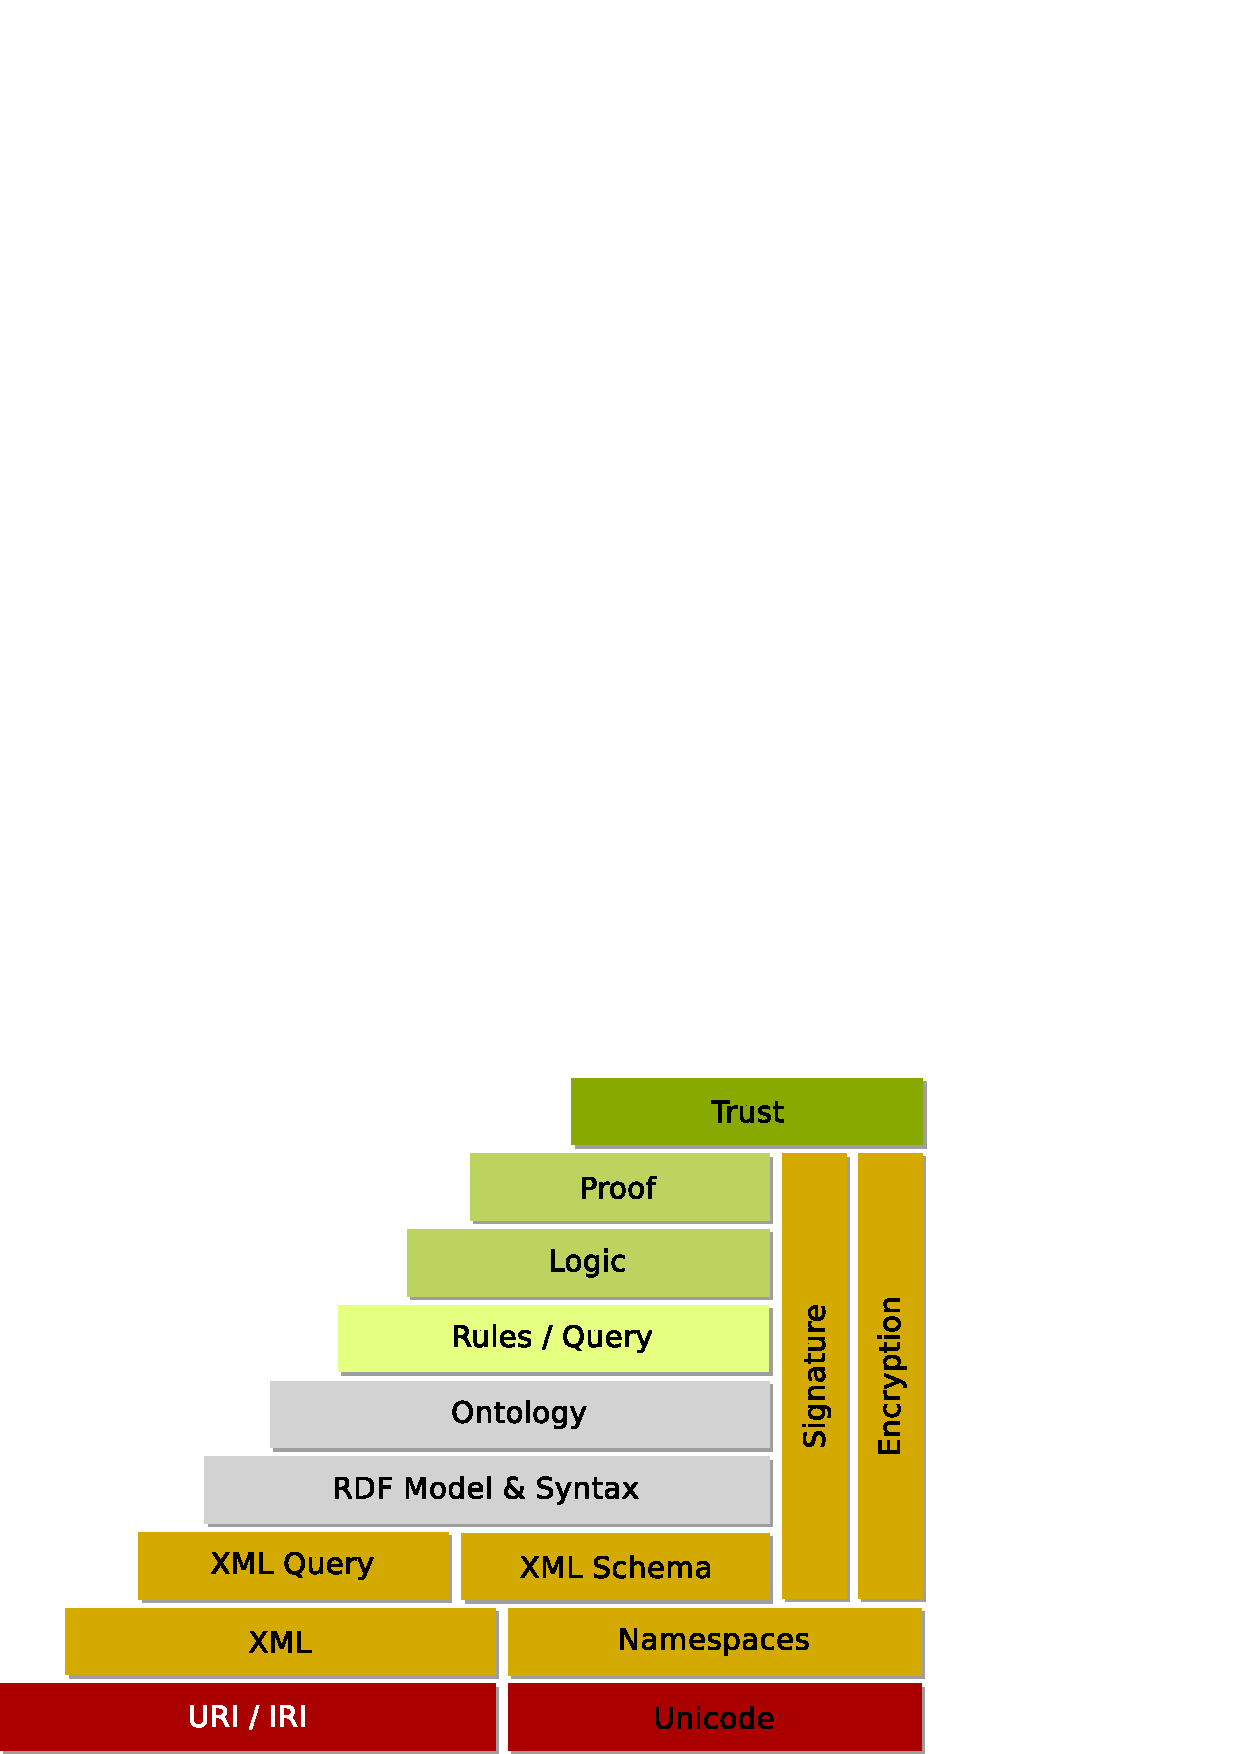
\includegraphics[width=0.6\textwidth]{img/pdf/w3c-semantic-web-layers.pdf}
% \begin{tablenotes}
% \item [1] In Zeile i: Die Differenz des Ähnlichkeitswertes zwischen Zeile i und Zeile i+1
% \end{tablenotes}
% \end{threeparttable}
% \caption[]{Die Komponenten des \emph{Semantic Web Stacks}}}
% \label{fig:semantic-web-stack}
% \end{figure}

\begin{figure}[htb]
    \begin{threeparttable}
    \centering  
    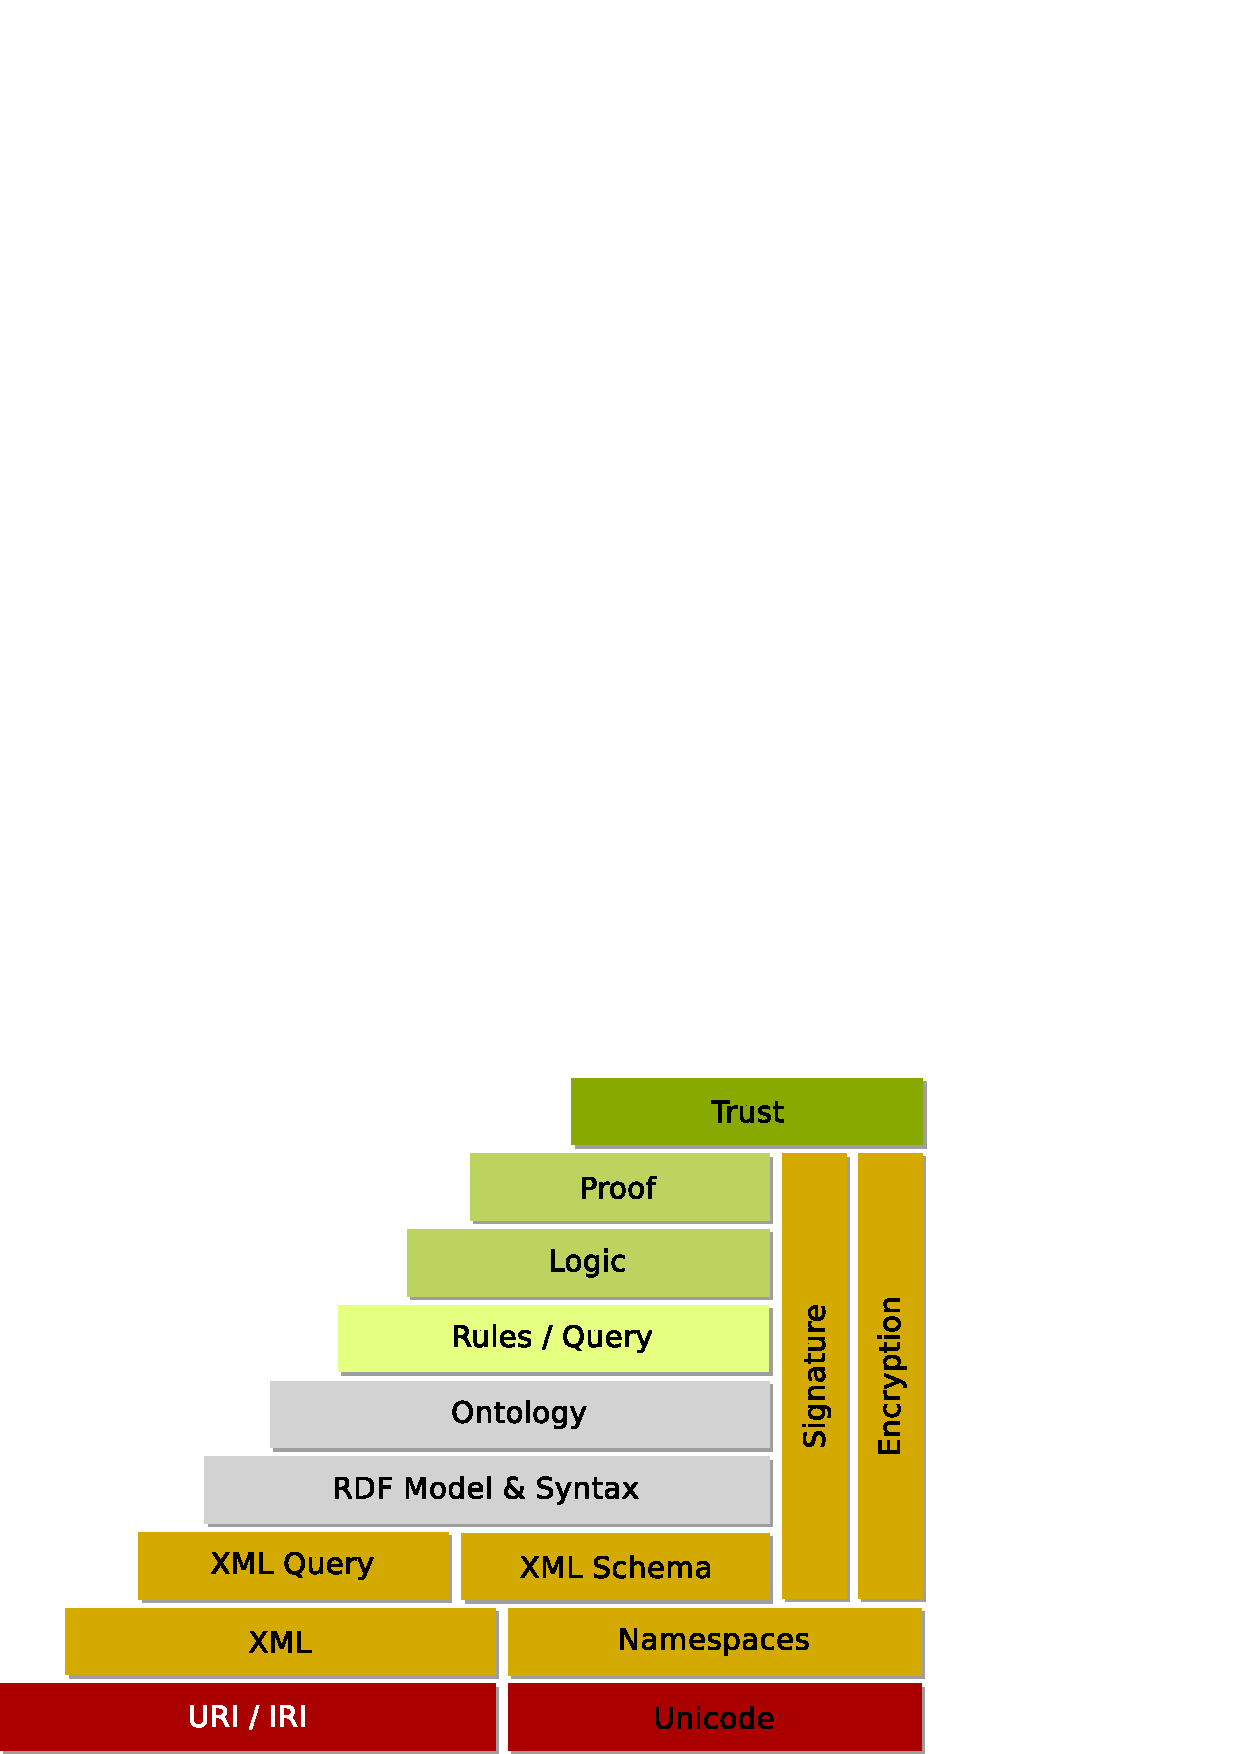
\includegraphics[width=0.6\textwidth]{img/pdf/w3c-semantic-web-layers.pdf}
      \begin{tablenotes}\footnotesize
      \item [~] Quelle: \url{en-wiki:File:W3c-semantic-web-layers.svg}
      \end{tablenotes}   
    \end{threeparttable}
    \caption[]{Die Komponenten des \emph{Semantic Web Stack}}
  \end{figure} 


\paragraph{}
Aus Platzgründen werden URIs oft mit Namensraum-Präfixen abgekürzt.
In dieser Arbeit ist beispielsweise \prefix{dbpedia} als Abkürzung für \url{http://dbpedia.org/resource/} definiert.
Dadurch können wir anstelle von \url{http://dbpedia.org/resource/London} nur \url{dbpedia:London} schreiben.
Die in dieser Arbeit verwendeten Namensraum-Präfixe befinden sich in Tabelle \ref{tab:namespace-prefixes}.
\paragraph{}
Es existieren folgende Unterarten von URIs:
\begin{itemize}
 \item \emph{Uniform Resource Locators (URLs)} identifizieren eine Ressource über ihren Zugriffsmechanismus. Sie sind also für eine Maschine erreichbare Ressourcen, wie zum Beispiel Webseiten.
Dies hat den Vorteil, dass zusätzliche Informationen über eine Ressource erhalten werden können, indem die URL dereferenziert wird.
\url{http://dbpedia.org/resource/London} dient also sowohl als eindeutige Identifikation als auch als Angabe, 
wie eine Maschine herausfinden kann, wie viele Einwohner London hat oder welche Flughäfen sich in der Stadt befinden.
 \item \emph{Uniform Resource Names (URNs)} sind dagegen dauerhafte, ortsunabhängige Ressourcenbezeichner mit dem Schema \emph{urn}. So identifiziert beispielsweise \url{URN:ISBN:0-671-43241-9} das Buch
\emph{The Hitchhiker's Guide to the Galaxy}, ohne jedoch anzugeben, wo man dieses Buch finden kann.
\end{itemize}
Ein Konzept kann sowohl durch eine oder mehrere URLs als auch durch eine oder mehrere URNs identifiziert werden.
Weiterhin gibt es URIs, die weder URLs noch URNs sind, zum Beispiel \url{mailto:max_mustermann@yahoo.com}.

\subsection{Das Resource Description Framework}
Das \emph{Resource Description Framework} (RDF, engl. (sinngemäß) „System zur Beschreibung von Ressourcen“) wird dazu genutzt, Informationen im Semantischen Web zu repräsentieren \citep{www-rdf}.
Es besteht aus einem \emph{semantischen Datenmodell}, um beliebige wahre Aussagen über Ressourcen zu treffen, und einem
grundlegendem \emph{Vokabular}, mit dem den Aussagen eine Bedeutung zugeordnet werden kann.
Da RDF für das Web gedacht ist, werden Konzepte mit URIs identifiziert.
Weiterhin unterstützt RDF anonyme Ressourcen und Literale wie Zeichenketten und Zahlen.
Eine Aussage in RDF ist ein Tripel aus \emph{Subjekt}, \emph{Prädikat} und \emph{Objekt}, die folgende Werte annehmen können:
\begin{center}
\begin{tabular}{lccc}
\toprule
		&URI		&Anonym			&Literal\\
\midrule
Subjekt		&\checkmark	&\checkmark\\
Prädikat	&\checkmark\\
Objekt    	&\checkmark	&\checkmark      	& \checkmark\\
\bottomrule
\end{tabular} 
\end{center}
Damit ähnelt eine RDF-Aussage einem stark vereinfachten deutschen Satz, zum Beispiel aus einer Leselernfibel.
Eine natürliche Sprache ist zwar ausdrucksstärker aber dafür nicht geeignet, denn sie ist inhärent mehrdeutig.\footnote{Beispiel: "`Ich habe nicht gesagt, sie hat das Geld gestohlen."'}
RDF nimmt also eine beschränkte Aussagekraft in Kauf, um eine möglichst einfache Verarbeitung zu ermöglichen.
Da ein Objekt eines Tripels das Subjekt eines anderen Tripels sein kann, lässt sich ein Tripel als Kante
in einem gerichteten, beschrifteten Graph auffassen.
Daher nennt man eine Menge von Tripeln auch einen \emph{Graphen}. 
Anonyme Ressourcen werden oft als \emph{blank nodes} bezeichnet.
\paragraph{Syntaxen}
Das RDF-Datenmodell ist eine abstrakte Syntax und damit unabhängig von einer bestimmten Darstellung.
Es gibt jedoch mehrere konkrete Syntaxen, wie zum Beispiel Turtle, RDF/XML und N3,  die in Ausdrucksstärke, menschlicher Lesbarkeit und Softwareunterstützung variieren.
Auch zum Speichern und Verwalten von RDF-Daten gibt es mehrere Möglichkeiten, \zb als Textdatei, auf einer Webseite oder in einem \emph{Triple Store}, dem RDF-Äquivalent einer Datenbank.

\begin{bsp}
Im vorigen Abschnitt wurden RDF-Statements mit den einfachen Sätzen in einer Leselernfibel verglichen.
Die folgenden drei Sätze lassen sich als Graph ausdrücken, indem für die Substantive und Verben URIs eingeführt werden:
\begin{itemize}
\item{"`Lilo mag Moni"'}
\item{"`Max sagt Ball"'}
\item{"`Susi sieht Sonne"'}
\end{itemize}
Als RDF-Graph:\\
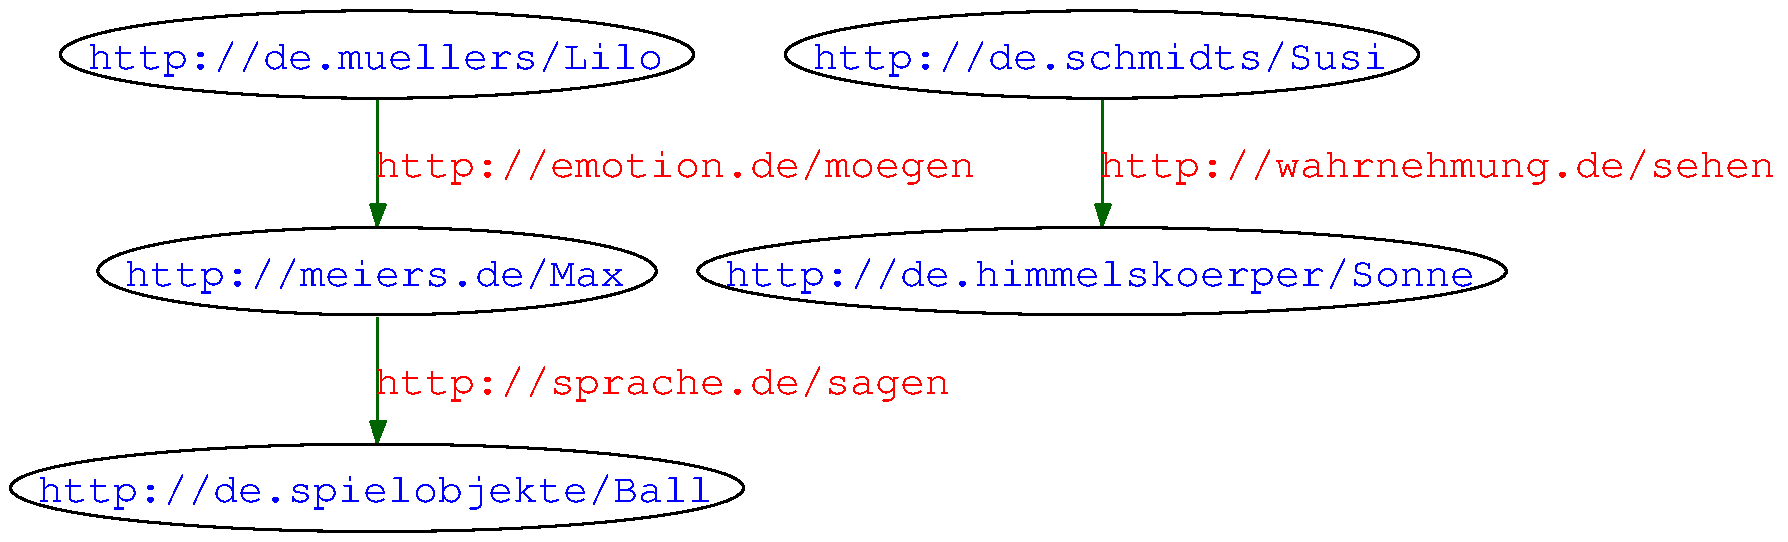
\includegraphics[width=\textwidth]{img/pdf/fibel_fontsize_20.pdf}\\
In N3:
\begin{itemize}
\item{\url{muellers:Lilo} \url{emotion:moegen} \url{meiers:Max}.}
\item{\url{muellers:Max} \url{sprache:sagen} \url{spielobjekte:Ball}.}
\item{\url{schmidts:Susi} \url{wahrnehmung:sehen} \url{himmelskoerper:Sonne}.}
\end{itemize}
 
\end{bsp}
% Um Information in einer für Maschinen verarbeitbaren Form darzustellen, benötigt man eine formale Sprache.
% 
% Weiterhin ist ihre Aussagekraft einfach zu groß.
% Es mag zwar paradox anmuten, dass eine große Ausdrucksfähigkeit einer Sprache zum Nachteil gereichen kann, doch erschwert sie die Validierung einer Aussage,
%  ja sie kann sie sogar unmöglich machen\footnote{Beispiel: "`Ich lüge jetzt."'}.
% Es muss also ein Kompromiß gefunden werden zwischen möglichst großer Ausdruckskraft auf der Einen und möglichst einfacher Verarbeitung der damit bildbaren Aussagen auf der anderen Seite.
% RDF nimmt dabei eine sehr beschränkte Aussagekraft in Kauf, um eine möglichst einfache Verarbeitung zu ermöglichen.
% Wenn wir eine möglichst einfache Untermenge unserer Sprache suchen, so erinnern wir uns sicher noch an unsere Grundschulzeit zurück und an das Lesenlernen mit einer Fibel.
% Die dort enthaltenen Sätze haben meist ein ganz einfaches Format:
% \begin{itemize}
% \item{"`Lilo mag Moni"'}
% \item{"`Max sagt Ball"'}
% \item{"`Susi sieht Sonne"'}
% \end{itemize}
% Sie besitzen ein Subjekt, ein Prädikat (Verb) und ein Objekt.
% Genau das ist RDF; da so eine Aussage aus genau drei Teilen besteht, spricht man auch von RDF-Tripeln.
% Allerdings sind die Bestandteile eines Tripels natürlich keine Wörter sondern URLs.
% Die drei Sätze würden also in RDF eher so aussehen:
% \includegraphics[width=\textwidth]{doc/latex/img/fibel_fontsize_20.ps}
% Ausgeschrieben:
% \begin{itemize}
% \item{\url{http://de.muellers/Lilo} \url{http://emotion.de/moegen} \url{http://de.meiers/Max}.}
% \item{\url{http://de.muellers/Max} \url{http://sprache/sagen} \url{http://de.spielobjekte/Ball}.}
% \item{\url{http://de.schmidts/Susi} \url{http://wahrnehmung/sehen} \url{http://de.himmelskoerper/Sonne}.}
% \end{itemize}
% Diese Notation nennt sich N3.


\iffalse
<?xml version="1.0"?>
<rdf:RDF  
xmlns:rdf="http://www.w3.org/1999/02/22-rdf-syntax-ns#"
xmlns:wahrnehmung="http://wahrnehmung.de/"
xmlns:emotion="http://emotion.de/"
xmlns:sprache="http://sprache.de/"
>
  <rdf:Description rdf:about="http://de.muellers/Lilo">
    <emotion:moegen rdf:resource="http://meiers.de/Max"/>
  </rdf:Description>
  <rdf:Description rdf:about="http://meiers.de/Max">
    <sprache:sagen rdf:resource="http://de.spielobjekte/Ball"/>
  </rdf:Description>
  <rdf:Description rdf:about="http://de.schmidts/Susi">
    <wahrnehmung:sehen rdf:resource="http://de.himmelskoerper/Sonne"/>
  </rdf:Description>
</rdf:RDF>
\fi
%Es gibt jedoch noch weitere Dateiformate, so kann man RDF genauso in einer Datenbank (Tripelstore) oder als XML (RDF/XML) abspeichern.

\subsection{SPARQL}
\emph{SPARQL} ist eine Abfragesprache für das Semantische Web \citep[siehe][]{www-sparql}.
Der Name ist ein rekursives Akronym für \emph{SPARQL Protocol and RDF Query Language}.
Der zentrale Part einer SPARQL-Anfrage besteht aus Tripelmustern, die mittels Konjunktionen und Disjunktionen miteinander verknüpft sind.
Diese Tripelmuster bestehen aus URLs und Variablen, die für das Subjekt, Prädikat und Objekt eines Tripels stehen.
Weiterhin muss die Abfrageart angegeben sein, welche die Werte \emph{SELECT}, \emph{CONSTRUCT}, \emph{ASK}, und
\emph{DESCRIBE} annehmen kann.
Einige SPARQL-Implementierungen definieren Erweiterungen für die SPARQL-Abfragesprache.
So bietet beispielsweise \emph{Virtuoso SPARQL} den Abfragemodus \emph{SELECT COUNT}, der nicht die zutreffenden Ergebnisse an sich, sondern nur deren Anzahl zurückgibt, was bei Anfragen dieses Typs 
einen deutlichen Geschwindigkeitsvorteil ermöglicht.
\begin{bsp}
\paragraph[]{Anfrage\footnote{\property{a} ist eine Abkürzung für \property{rdf:type}}}
\begin{verbatim*}
SELECT ?o WHERE
{
<http://dbpedia.org/resource/Ant> a ?o.
} 
\end{verbatim*}
\paragraph{Ergebnis}
\begin{verbatim*}
owl:Thing
<http://sw.opencyc.org/2008/06/10/concept/Mx4rvVjf5JwpEbGdrcN5Y29ycA>
dbpedia:ontology/Species
dbpedia:ontology/Animal
dbpedia:ontology/Insect
dbpedia:ontology/Eukaryote
\end{verbatim*}

\end{bsp}

\subsection{Linked Data}
Eine Webseite, die keine Links enthält und auf die nicht verlinkt wird, ist nutzlos.
Sie wird von einer Suchmaschine nicht gefunden und auch wenn man einen Artikel über ein ähnliches Thema liest, erfährt man nicht von der Existenz dieser Seite.
Das zentrale Element des WWW ist also die Verknüpfung durch Links. Diese sind jedoch nicht \textit{typisiert}, das heißt ein Link gibt nur an, dass irgendeine Art Beziehung existiert, aber nicht, welche das genau ist.
Ein menschlicher Benutzer kann anhand der Beschreibung im Text entscheiden, welchen Links er folgt und welchen nicht. 
Dies stellt jedoch ein enormes Problem für einen Agenten dar, der eine bestimmte Information sucht und herausfinden muss, welche der Links für ihn relevant sind.
\emph{Linked Data} löst dieses Problem, indem jeder Link zwischen zwei Entitäten einen bestimmten Typ hat.
%Analog dazu wird das enorme Potential des Semantischen Webs erst dann ausgereizt, wenn die darin enthaltene Information sinnvoll miteinander verknüpft wird.
Das Konzept geht auf einen Vorschlag von \citet{www-linked-data-proposal} zurück und legt auch die zu benutzenden Technologien fest.
Grundprinzipien sind:\footnote{Aus dem Englischen übersetzt aus \cite{www-linked-data-proposal}.}
\begin{enumerate}
\item{Benutze URIs als Namen für Dinge}
\item{Benutze HTTP URIs, damit menschliche Benutzer den Namen nachschlagen können}
\item{Stelle nützliche Information über eine URL in Form der Standards RDF und SPARQL zur Verfügung}
\item{Verlinke auf andere URIs, sodass der Benutzer andere Dinge entdecken kann}
\end{enumerate}
Während im WWW die Links, die von einem Dokument auf ein Anderes verweisen, in Ersterem enthalten sein müssen, kann Jedermann Linked Data über Dinge seiner Wahl bereitstellen,
und damit Verknüpfungen zwischen bereits existierenden Ressourcen erschaffen.
\iffalse
Je größer das Netzwerk und der Vernetzung dazwischen, desto wertvoller ist jede einzelne Ressource. Dies führt zu einem superlinearen Wachstum 
So wie ein Student, der sich stur Fakten um Fakten einverleibt, keinen Erfolg haben wird\footnote{Im Fachbereich Informatik jedenfalls\ldots},

Das Semantische Web besitzt ein beeindruckendes Potential.
Die Zahl der möglichen Anwendungen, die Auswirkungen auf die Informationstechnik und die vorstellbaren Veränderungen im Alltag jedes Einzelnen sind zwar gewaltig (im Guten wie auch im Bösen), 
doch leidet das Semantische Web an einem prinzipiellen Problem von Netzwerken:
Der Nutzen eines Netzwerkes für jeden Teilnehmer wächst mit der Größe des Netzwerkes. Zu Beginn ist der Anreiz, 
-> Metcalfesches Gesetz
Schier überwältigend ist die Zahl der möglichen Anwendungen des Semantischen Webs, des mögli
\fi

\subsection{Ontologie}
Eine \textit{Ontologie} ist eine formale Beschreibung einer Menge von Konzepten und der Beziehungen dieser Konzepte untereinander.
Eine Ontologie stellt ein gemeinsames Vokabular für ein bestimmtes Fachgebiet zur Verfügung und erlaubt es, Aussagen über die Merkmale dieses Fachgebietes zu treffen oder es zu definieren. 
%Sie beschreibt, welche Arten von Objekten und Konzepten existieren und wie diese zusammenhängen.
Eine Ontologie hat folgende Bestandteile:
\begin{itemize}
\item \emph{Instanzen} oder \emph{Individuen} sind die grundlegenden Objekte in der Ontologie, \zb{} \emph{London}.
\item \emph{Klassen} oder \emph{Typen} sind Mengen von Instanzen. \emph{London} ist ein Element der Klasse \emph{Stadt},
im Folgenden auch "`\emph{London} ist eine Instanz der Klasse \emph{Stadt}"' oder "`\emph{London} ist vom Typ \emph{Stadt}"'.
\item \emph{Literale} sind Werte wie Zahlen oder Zeichenketten.
\item \emph{Relationen} oder \emph{Properties} beschreiben die Beziehungen zwischen Klassen, Instanzen und Literalen.
\item \emph{Axiome} sind wahre Aussagen innerhalb der Ontologie die Wissen repräsentieren, \zb{} "`Zwischen London und Leipzig existiert eine Zugverbindung"'.
\end{itemize}

%Eine Ontologie über die grammatikalische Struktur von Sätzen könnte unter anderem definieren, dass ein \emph{Satz} aus \emph{Hauptsätzen} und \emph{Nebensätzen} \emph{besteht}, ein \emph{Hauptsatz} ein \emph{Subjekt} und ein \emph{Prädikat} \emph{enthält} und dass ein \emph{Personalpronomen} ein \emph{Pronomen} \emph{ist}.
Ontologien werden durch spezielle Beschreibungssprachen repräsentiert. 
Dabei existieren einige solcher Sprachen, wie \textit{RDFS}, \emph{OWL Lite}, \emph{OWL DL}, \emph{OWL Full} und \textit{OWL 2}, die sich in Ausdrucksstärke, Komplexität und Entscheidbarkeit unterscheiden.
Während es in RDFS beispielsweise erlaubt ist, das Klassen Instanzen von anderen Klassen sind, ist dies in OWL DL nicht möglich.
\iffalse
\paragraph{OWL}
OWL (Web Ontology Language) ist eine Beschreibungssprache für Ontologien. Sie verwendet die Syntax von RDF und lässt sich in drei verschiedenen Versionen benutzen.
\begin{itemize}
\item{OWL Lite}
\item{OWL DL}
\item{OWL Full}
\end{itemize}
Die hier verwendete Version ist OWL \todo{[insert here]}.
blabla
\fi

\subsection{Open World Assumption}
Liegt einem Auskunftssystem alle vorhandene Information über ein bestimmtes Thema vor, dann kann dies alle Anfragen, ob eine bestimmte, in diesem System formulierbare, Aussage gültig ist oder nicht, mit entweder ja oder nein beantworten.
Wenn ein Kinobesucher wissen möchte, ob er sich Freitag Abend \emph{Twilight -- New Moon} ansehen kann und im Spielplan zu dieser Zeit kein Eintrag existiert, dann kann ihm der Mitarbeiter mit Sicherheit sagen,
dass sich der Kunde diesen Film zu dieser Zeit leider nicht ansehen kann.
Dem Kinospielplan liegt also eine \emph{Closed World Assumption} (Geschlossene-Welt-Annahme) zugrunde.
Im Semantischen Web wird jedoch Weltwissen repräsentiert, welches an vielen verschiedenen Orten gespeichert und niemals vollständig ist.
Aussagen die nicht explizit vorliegen können also nicht bestätigt, jedoch auch nicht verneint werden.
Es gilt also die \emph{Open World Assumption} (Offene-Welt-Annahme).

%\subsection{Der DL-Learner}
%Der DL Learner\footnote{Projektseite \url{http://dl-learner.org/Projects/DLLearner}} ist ein Programm, welches Konzepte in Beschreibungslogiken, wie OWL, anhand von Beispielen lernt. Bei Eingabe von positiven und negativen Beispielen erzeugt er ein passendes OWL-Konzept, es sind jedoch auch andere Betriebsmodi möglich.
%Er ist in Java implementiert und steht unter einer Open Source Lizenz und ist damit sehr gut in andere Javaprogramme integrierbar.

\section{Grundbegriffe der Linguistischen Informatik}

Ein \definition{Parser} für natürliche Sprache ist ein Programm, dass die grammatikalische Struktur von Sätzen (die \emph{Morphologie}) bestimmt.
Ein Satz könnte beispielsweise in einen Hauptsatz und einen Nebensatz unterteilt werden, ein Wort als Subjekt gekennzeichnet werden, ein anderes als Objekt und ein weiteres als Verb.
Da die Grammatik einer natürlichen Sprache kompliziert und im allgemeinen NP-vollständig ist, sind die meisten Parser statistisch.
Statistische Parser benutzen als Trainingsmenge Texte einer bestimmten Sprache -- ein \definition{Korpus} -- die mit einer Menge von Tags -- einem \definition{Tagset} -- annotiert wurden.
Ein solches annotiertes Korpus nennt man auch \definition{Treebank}.

Ein Programm, das Sätze in seine Einzelteile (Tokens), dies sind Wörter und Satzzeichen, zerlegt, heißt \definition{Chunker}. %\footnote{Im Allgemeinen wird darunter auch die Identifizierung von Satzbestandteilen verstanden.}.
Ein \definition{Feature} bezeichnet eine beliebige Eigenschaft eines Satzes, zum Beispiel ob er ein ein Aktiv- oder ein Passivsatz ist oder ein Reflexivpronomen enthält.
Die \definition{Grundform} oder das \definition{Lemma} eines Wortes ist die Form, unter der man es in einem Nachschlagewerk findet
(ein Beispiel: \emph{getrunken} $\rightarrow$ \emph{trinken}).
Die \emph{Stammform} (englisch \emph{stem}) hingegen ist der Kern eines Wortes, der als Basis zur Bildung der gebeugten Wortform dient.
Der Stamm von \emph{trinken} wäre also \emph{trink}, aus dem sich dann die Formen \emph{trinke}, \emph{trinkst}, \emph{trinken}, \emph{trinkt} bilden lassen.

\iffalse
\paragraph{Textklassifikation}
Das Problem der Textklassifikation besteht darin, einen Satz oder ein elektronisches Dokument automatisch in eine oder mehrere Kategorien einzuteilen.
Man unterscheidet dabei zwischen überwachter, halbüberwachter und unüberwachter Klassifikation,
 je nachdem ob und in welchem Maß eine externe Quelle (\zb{} ein Mensch) Informationen über die korrekte Klassifikation beisteuert.
In dieser Arbeit sind diese Kategorien nur "`weist Merkmal x auf"' und "`weist Merkmal x \emph{nicht} auf"'.
\fi
\section{Wikipedia}
Wikipedia ist eine freie, Wiki-basierte Online-Universalenzyklopädie, die von DBpedia als primäre Datenquelle benutzt wird.
Durch die \emph{Creative-Commons-Lizenz} ist sie nicht nur kostenlos verfügbar sondern darf auch frei kopiert und verwendet werden.

\paragraph{Wiki}
ist das hawaiische Wort für schnell und bezeichnet eine Technik, die es einer großen Menge von Benutzern ermöglicht, gemeinsam Internetseiten zu erstellen.
Dabei gibt es sowohl firmeninterne, als auch frei zugängliche Wikis.
Der Durchbruch der Konzepts kam mit Wikipedia, mittlerweile gibt es jedoch viele weitere wiki-basierte Projekte, zum Beispiel Wikibooks und Wiktionary.
Das grundlegende Konzept ist, dass Benutzer Seiten ansehen und editieren können.
Trotz anfänglicher Befürchtungen hat sich dieser Ansatz aufgrund der aktiven Gemeinschaft als erstaunlich robust herausgestellt.
So wird beispielsweise die Hälfte aller Massenlöschungen in weniger als drei Minuten wieder rückgängig gemacht \citep[Seite 579]{wikipedia-vandalism}.
Sämtliche Versionen sind in einer Chronik gespeichert und können jederzeit wiederhergestellt werden.
Die Versionierung hat jedoch noch einen weiteren Vorteil:
So dienen ältere Versionen als dauerhafte Abbilder eines Artikels zu einem bestimmten Zeitpunkt.
In dieser Arbeit sind Verweise auf Seiten der Wikipedia deshalb mit ihrer Versionsnummer versehen.
Auch die Qualität des gemeinschaftlichen Ansatzes hat sich als hoch genug erwiesen, dass bereits gerichtliche Entscheidungen auf Basis von in Wikipediaartikeln enthaltenen Informationen gefällt wurden \citep*{wikipedia-formula-one}.

\paragraph{Artikel}
Der elementare Baustein von Wikipedia ist der Artikel.
Jeder dieser Artikel beschreibt ein bestimmtes Konzept, welches sowohl eine Klasse (\article{en-wiki:Human}) als auch eine Instanz (\article{en-wiki:Al_Pacino}) sein kann.
%Welche Arten von Konzepten jedoch genau durch Artikel beschrieben werden ist jedoch schwer zu definieren.
%Die Seite \article{en-wiki:Wikipedia:What is an article}\footnote{\url{http://en.wikipedia.org/w/index.php?title=Wikipedia:What_is_an_article?&oldid=347855498}} 
%nur "`A Wikipedia article is a page that has encyclopedic information on it"'.
In Abgrenzung von einem Wörterbuch ist ein enzyklopädischer Artikel in Wikipedia folgendermaßen beschrieben:\footnote{\url{http://en.wikipedia.org/w/index.php?title=Wikipedia:Wikipedia_is_not_a_dictionary&oldid=353213935}}
\begin{quote}
Each article in an encyclopedia is about a person, or a people, a concept, a place, an event, a thing etc.; whereas a dictionary article is primarily about a word, an idiom or a term and its meanings, usage and history.
\end{quote}

Als Abgrenzung eines Artikels zu einer anderen Seite der Wikipedia existiert die Definition:
"`Ein Artikel ist eine Seite, die im Artikelnamensraum liegt (kein Präfix), keine Weiterleitung ist und mindestens einen Wikilink enthält."'\footnotemark{}
\footnotetext{Übersetzt aus {\url{http://en.wikipedia.org/w/index.php?title=Wikipedia:What_is_an_article?&oldid=347855498}}}
Dies schließt auch Disambiguierungsseiten ein, die meist nur aus Wikilinks und deren Kurzbeschreibungen bestehen.
\paragraph{} 
Der Name eines Artikels auf ist gleich seinem Titel, wobei jedoch Leerzeichen durch Unterstriche ersetzt werden.
Ist der Artikel eine Disambiguierungsseite, dann wird der Name meist um ein "`\_(Disambiguation)"' (bzw. das Äquivalent in anderen Sprachversionen) erweitert.
Gibt es mehrere gleichnamige Artikel, dann wird sowohl an den Titel als auch an den Artikelnamen in Klammern der Kontext angehängt; wird eine Bedeutung im Sprachgebrauch jedoch häufiger benutzt,
kann dieser auch keine Klammern enthalten.
Ein Beispiel hierfür sind die Artikel \emph{Bank\_(Begriffsklärung)}, \emph{Bank} (dieser Artikel beschreibt das Kreditinstitut) und \emph{Bank\_(Möbel)}.
% "`A good encyclopedia article can and should begin with a relatively short but discrete explanation of what the subject of the article — the person, place, concept, event, or thing that its title denotes — is."'
% "`Wikipedia articles should begin with a good definition and description of one topic, however, they should provide other types of information about that topic as well."'
% http://en.wikipedia.org/w/index.php?title=Wikipedia:Wikipedia_is_not_a_dictionary&oldid=353213935
%\paragraph{Qualität}
%Während dies bei einem normalen Artikel noch nicht dem Anspruch einer zitierfähigen Quelle gerecht wird, kann bei Seiten des 
%In Wikipedia gibt es zu jedem Artikel eine Diskussionsseite, in der über geplante Änderungen diskutiert wird.
%Entscheidungen werden in einem gemeinsamen Prozess gefällt.

\section{DBpedia}
Das \textit{DBpedia}-Projekt extrahiert strukturierte Informationen aus Wikipedia-Artikeln und 
stellt diese frei im Web zu Verfügung. 
DBpedia ist also der Semantic-Web-Gegenpart zu Wikipedia.
Die durch das Projekt generierten RDF-Daten repräsentieren eine Teilmenge der in den Wikipedia-Artikeln enthaltenen Informationen.
Die extrahierten Daten sind mit der zu diesem Zweck erstellten DBpedia-Ontologie klassifiziert. Durch das \emph{Linking Open Data}-Projekt wurde DBpedia jedoch auch mit den
Wissensquellen YAGO und Open-Cyc verlinkt, wodurch zusätzliche Klassifikationsschemata bereitstehen.
%Die Daten werden dann als Linked Data und über SPARQL-Interfaces veröffentlicht.
Die große Errungenschaft von DBpedia ist, dass sie einen Teil der unermesslichen Informationsfülle von Wikipedia
für das Semantische Web zur Verfügung stellt und damit den Nutzen vieler Anwendungen erhöht oder sie erst möglich macht.
Dies macht DBpedia zu einer der zentralen Verknüpfungsstellen der \emph{LOD-Cloud}, der Menge der vom \emph{Linking Open Data Project} \citep{lod} verlinkten Wissensquellen, und leistet damit einen entscheidenden Beitrag, um das Wachstum des Semantic Web in Gang zu bringen.
\begin{figure}[h]
\begin{center}
\begin{threeparttable}
\includegraphics[width=\textwidth]{img/pdf/lod-cloud.pdf}
\begin{tablenotes}
\item [] \begin{footnotesize} Quelle: \url{http://richard.cyganiak.de/2007/10/lod/lod-datasets_2009-07-14.pdf}\end{footnotesize}
\end{tablenotes}
\end{threeparttable}
\end{center}
\caption{die LOD-Cloud}
\end{figure}
Die Daten von DBpedia sind via Download, \emph{Virtuoso SPARQL}- und Linked Data-Interface verfügbar.
Abbildung \ref{fig:dbpedia-pig} zeigt eine DBpedia-Entität als HTML-Sicht des Linked Data-Interfaces.
Die drei wesentlichen Bestandteile des DBpedia-Projektes sind die Webseite, die Datensets und das Extraktions-Framework.
Unter den Datensets ist jenes, das aus der englischen Wikipedia extrahiert wurde das Wichtigste.
Darin existiert zu jedem Wikipedia-Artikel \article{en-wiki:Articlename} eine RDF-Entität \article{dbpedia:Articlename}.
Informationen aus den entsprechenden Artikeln anderer Sprachversionen werden jedoch auch unter dem Namen des englischen Artikels von der DBpedia zur Verfügung gestellt.
\iffalse
The DBpedia ontology has been created for the purpose
of classifying this extracted data. In the course of the Linking Open Data project, DBpedia be-
came interlinked with other knowledge bases, namely YAGO, SKOS, UMBEL and Open-Cyc,
serving as additional classification schemata. This step cleared the path for DBpedia to become
one of the most important linking hubs within the LOD-cloud.
\fi
%Notably the latter two are powered by OpenLink’s Virtuoso Universal Server. -> eigentlich nicht interessant hier
%fig:dbpedia-pig

\iffalse
\section{LOD-Cloud}
\begin{quote}
Linked Data is about using the Web to connect related data that wasn't previously linked, or using the Web to lower the barriers to linking data currently linked using other methods.
More specifically, Wikipedia defines Linked Data as
"`a term used to describe a recommended best practice for exposing, sharing, and connecting pieces of data, information, and knowledge on the Semantic Web using URIs and RDF."'
\end{quote}

-> \todo{ein ordentliches eps finden}
\begin{center}
\includegraphics[width=\textwidth]{img/pdf/lod-cloud.pdf} 
\end{center}
\fi

\iffalse
\subsection{Mathe}
Zu (i) folgenden Lösungsansatz:
Seien $ w_1, w_2 \in W*, v \in V* $
$ f*(w_1 + w_2)(v) = (w_1 + w_2)(f)(v) = (w_1 \circ f)(v) + (w_2 \circ f)(v) = f*(w_1)(v) + f*(w_2)(v) $
$ \Rightarrow f*(w_1) + f(w_2) $

------------
Zu (ii)
Zz.: $ ker(f*) = im(f)^\perp $

$ ker(f*) \subseteq im(f)^\perp $
Sei $ l \in ker(f*) $ und $ v \in V $
$ \Rightarrow f*(l)(v)=0 \forall v \in V $
$ \Rightarrow (l \circ f)(v)=0 \forall v \in V $
$ \Rightarrow l(f(v))=0 \forall v \in V $
$ \Rightarrow l(w)=0 \forall f(v)=w \in W $
$ \Rightarrow l \in im(f)^\perp $

$ ker(f*) \supseteq im(f)^\perp $
$ \Rightarrow l(w)=0 \forall w \in W $
$ \Rightarrow l(f(v))=0 \forall v \in V $
$ \Rightarrow (l \circ f)(v)=0 \forall v \in V $
$ \Rightarrow f*(l)(v)=0 \forall v \in V $
$ \Rightarrow l \in ker(f*) $
\fi

\subsection{Grundbegriffe der Graphentheorie}
Mit $[A]^k$ bezeichnen wir die Menge aller k-elementigen Teilmengen von A.
Ein \emph{Graph} ist ein Paar $G = (V, E)$ disjunkter Mengen (von \emph{Ecken} und \emph{Kanten}) mit $E \subseteq [V]^2$; die Elemente von E sind also 2-elementige Teilmengen von V.
Ein Graph, der keinen Kreis enthält, ist ein \emph{Wald}.
Ein zusammenhängender Wald ist ein \emph{Baum}.
Einen \emph{Baum} mit fest gewählter Wurzel nennt man einen \emph{Wurzelbaum}.
Ein gerichteter Graph ist ein Paar $(V, E)$ disjunkter Mengen zusammen mit zwei Funktionen
init$: E \rightarrow V$ und 
ter$: E \rightarrow V$, die jeder Kante $e$ eine Anfangsecke init$(e)$ und eine Endecke ter(e) zuordnen;
die Kante $e$ heißt dann von init$(e)$ nach ter$(e)$ gerichtet.
Die obigen Definitionen stammen aus \citet{graphentheorie}.
Ein gerichteter Graph, der keinen Kreis enthält heißt auch \emph{DAG} (engl. \emph{directed acyclic graph}).
Ein \emph{gerichteter Wurzelbaum} ist ein zusammenhängender DAG mit einer fest gewählten Wurzel.
Es gibt zwei Arten von gerichteten Wurzelbäumen: bei \emph{Out-Trees} ist jeder Knoten über einen Pfad von der Wurzel aus erreichbar, bei \emph{In-Trees} ist die Wurzel über einen Pfad von jedem Knoten aus erreichbar.

\subsection{Grundbegriffe der Ordnungstheorie}
Eine Halbordnung ist eine zweistellige Relation "`$\leq$"' auf einer Menge M mit folgenden Eigenschaften:%$\leq\ \subseteq M \times M$
\begin{center}
\begin{tabular}{ll}
\toprule
Reflexivität	&$x \leq x, \forall x \in M$\\
Transitivität	&$(x \leq y \land y \leq z) \rightarrow (x \leq z), \forall x,y,z \in M$\\
Antisymmetrie	&$(x\leq y \land y\leq x) \rightarrow x=y, \forall x,y \in M$\\
\bottomrule
\end{tabular} 
\end{center}
$x < y$ ist eine Abkürzung für $x \leq y \land x \neq y$.
%Eine Relation $R$ ist \emph{reflexiv}, wenn gilt $x \leq x, \forall x \in M$, \emph{transitiv}, wenn gilt $(x \leq y \land y \leq z) \rightarrow (x \leq z), \forall x,y,z \in M$) und antisymmetrisch, wenn gilt $(x\leq y \land y\leq x) \rightarrow x=y, \forall x,y \in M$.
%Wichtige Eigenschaftsbegriffe für Relationen sind:
Zu einer beliebigen zweistelligen Relation $R \subseteq M \times M$ lässt sich die \emph{transitive Hülle} $R^+$ bestimmen, die die Relation $R$ um die Paare erweitert, die zur Einhaltung der Transitivität nötig sind.
Sie ist definiert als: $x \ R^{+} \ y : \Leftrightarrow \exists n \geq 0 \ \exists e_1,\dots ,e_n \in V: x \,R \,e_1 \,R \,e_2 \,R \dots \,R \,e_n \,R \,y$.


\subsection{Hierarchien in DBpedia}\label{sec:grundlagen-hierarchien}
Eine Hierarchie ist eine Anordnung von Klassen, welche einander über- oder untergeordnet sind.
Ist Klasse $A$ Klasse $B$ übergeordnet, dann heißt $A$ "`\emph{Superklasse} von $B$"' und $B$ "`\emph{Subklasse} von $A$"'.
Ist ein Individuum Instanz einer Klasse, dann ist es auch Instanz deren Superklassen.\footnote{Hierarchien, in denen Klassen welche selbst wieder Instanzen von Klassen sein können, werden in dieser Arbeit nicht betrachtet.}
Die Subklassenrelation entspricht also der Teilmengenrelation $\subseteq$ und ist damit eine Halbordnung.
%Die Superklassenrelation enhält dann das Paar $(A,B)$, die Subklassenrelation das Paar $(B,A)$.
In der Praxis wird nur die Relation der direkten Subklassen verwaltet, die Subklassenrelation ist dann die transitive Hülle der direkten Subklassenrelation.
Dieses Verfahren kann auch bei der Klassenzugehörigkeit eines Individuums angewandt werden, eine vollständige Angabe der Klassenzugehörigkeit heißt auch \emph{expandiert}.
%Aus Gründen der Speicherplatz-, Rechenzeit- und Darstellungsplatzersparnis werden im praktischen Einsatz nur die direkten Sub- oder Superklassen angegeben und verwaltet, die Super- und Subklassenrelationen sind dann die transitiven Hüllen super$^+$ und sub$^+$ der direkten Sub- und Superklassenrelationen super und sub.
%Da die Teilmengenrelation $\subseteq$ eine Halbordnung ist, ist der Graph der Sub- und Superklassenrelation 
%Der Graph der direkten Sub- und Superklassenrelation entspricht dann der \emph{Minimalrepräsentation}, also der \emph{transitiven Reduktion} dieses Graphen und ist damit auch ein DAG.
Besitzt die Hierarchie eine \emph{Wurzel}, dann gibt es eine allen Klassen gemeinsame Oberklasse.%, es gilt also super$^+(O,K)$ für alle Klassen $K$.
Ein Spezialfall der Hierarchie ist die \emph{Monohierarchie}, bei der die direkte Subklassenrelation einen In-Tree bildet,
eine \emph{Polyhierarchie} bezeichnet eine Hierarchie, bei der dies nicht der Fall sein muss.% Bei einer Polyhierarchie ist es also möglich, dass ein 

%Ein Spezialfall der Hierarchie ist die \emph{Monohierarchie}, bei der die direkte Sub- und Superklassenrelation einen gerichteten Wurzelbaum bildet.
%Bei der Angabe der Klassenzugehörigkeit einer Entität können enweder nur die unmittelbar zugeordneten oder sämtliche übergeordneten Klassen angegeben werden, der letztere Fall wird im Folgenden auch als \emph{expandierte Klassenzugehörigkeit} benannt.
%Eine Hierarchie, die keine Monohierarchie ist, heißt auch \emph{Polyhierarchie}.

%Besitzen manche Elemente mehrere direkte Superklassen, handelt es sich um eine \emph{Polyhierarchie}.
\iffalse
\begin{dfn}
Eine Hierarchie ist ein DAG $G = (V,\subseteq)$, wobei $V$ die Menge der \emph{Klassen} und $\subseteq$ die Superklassenrelation ist.
Es gilt also: $(e_1,e_2) \in E$ gdw. $e_1$ ist eine Superklasse von $e_2$.
%Dabei existiert genau eine Wurzel, das heißt eine Klasse, welche keine Superklasse besitzt.

Eine Monohierarchie ist sogar ein Baum.
\end{dfn}
\fi
\paragraph{Wikipediakategorien}%SKOS
In der Wikipedia kann jeder Artikel durch die Benutzer manuell einer oder mehreren Kategorien zugeordnet werden.
Diese Kategorien können nun selbst wieder Kategorien zugeordnet werden und bilden annähernd eine Polyhierarchie mit einer einzelnen Wurzel \url{Contents}.
%Das Kategoriensystem der Wikipedia ist also ein Thesaurus, das heißt eine Menge von Schlüsselwörtern, die mit Relationen (in diesem Fall \emph{ist Unterkategorie von } und \emph{ist Oberkategorie von}) verbunden sind.
Aufgrund der großen Menge an Kategoriendaten\footnotemark{} sind zu fast jedem Artikel semantische Daten verfügbar.
\footnotetext{Zum Zeitpunkt dieser Arbeit sind es 410618 Zuordnungen}
Da sich die Kategorien jedoch nicht nur auf die Artikelgegenstände, sondern auch auf die Artikel selbst beziehen können, sind nicht alle davon für einen
taxonomischen Vergleich der Artikelgegenstände nützlich, so \zb{} \emph{Wikipedia:Gesprochene\_Artikel} oder \emph{Wikipedia:Exzellent}.
Weiterhin sind die Daten teilweise unsauber, sodass Zyklen enthalten sind.

\paragraph{YAGO}
\citep[beschrieben in][]{yago} ist eine Polyhierarchie mit einer einzigen Wurzel namens \url{Entity} und verbindet die große Anzahl von Konzepten der Wikipedia mit der sorgfältig gepflegten Hierarchie von WordNet \citep{wordnet} um eine hochqualitative Hierarchie zu erzeugen.
Dabei enthält YAGO über \val{150000} Klassen.%Relationen, wobei sowohl Taxonomische ("`ist ein"') als auch nichttaxonomische Relationen enthalten sind.
%159375
\paragraph{DBpedia-Klassen}%owl-ontology
Eine weitere Hierarchie basiert auf der Extraktion von Klassen aus Wikipedia-Infoboxen.
So wird manuell einigen Infoboxtypen eine zugehörige Klasse zugeordnet.
Weist ein Artikel beispielsweise die Infobox "`Filmdaten"' auf, so wird dieser Artikel der Klasse \url{http://dbpedia.org/ontology/Film} zugewiesen.
Diese von Hand erstellte Hierarchie enthält nur 199 Klassen und bildet eine Monohierarchie mit der Wurzelkategorie \url{owl:Thing}. Die zugehörigen Daten sind sehr präzise, da Infoboxtypen sehr spezifisch sind.
 
\section{Projekt Deutscher Wortschatz}\label{sec:wortschatz}
Das \emph{Projekt Deutscher Wortschatz} der Universität Leipzig bietet statistische Informationen über Wörter aus einer Vielzahl von Sprachen
und wurde 1994 unter der Leitung von Uwe Quasthoff gestartet.
Mit je über 9 Millionen Sätzen ist das Wortschatzkorpus eines der größten Korpora in Deutsch, Englisch und Italienisch,
weiterhin existieren noch kleinere Korpora in anderen Sprachen.
Die gespeicherten Sätze stammen "`zum größten Teil aus Zeitungstexten, zu einem geringeren Teil auch aus
Fachtexten oder speziellen Wortlisten"' \cite[Seite 1]{wortschatz}.
Aus urheberrechtlichen Gründen werden die Texte jedoch satzweise und nicht als ganzer Artikel verwaltet.
Zu jeder Wortform ist eine Vielzahl an Informationen verfügbar, unter anderem die \emph{Frequenz}, \emph{Frequenzklasse}, \emph{Nachbarn}, \emph{Kookurrenzen} und \emph{Beispielsätze}.
In dieser Arbeit wird sowohl die Frequenz als auch die Frequenzklasse genutzt.
\paragraph{}
Die \textbf{Frequenz} bestimmt die Häufigkeit eines Wortes, sie ist definiert als die Anzahl der Sätze im Korpus, in denen die Wortform vorkommt.
\paragraph{}
Die \textbf{Frequenzklasse} bestimmt die Seltenheit eines Wortes und ist eine ganzzahlige Funktion der Frequenz; sie steigt wenn diese fällt.
Die häufigsten Wörter haben die Frequenzklasse 0, während die seltensten Wörter in der größten Frequenzklasse liegen.
Dabei macht man sich zunutze, dass in natürlichen Sprachen einige wenige Wörter sehr häufig, sehr viele Wörter jedoch sehr selten vorkommen.
Abbildung \ref{fig:zipf_wortschatz} zeigt, wie sich die Verteilungen der Frequenzen der Wörter von zwei Korpora des Wortschatzes verhalten.
Es kann nachgewiesen werden (hier exemplarisch an einem 1 Million Sätze großen englischen Normkorpus), dass sie dem \emph{Zipfschen Gesetz} \citep{zipf} entsprechen.
Es besagt: Ordnet man die Elemente absteigend nach ihrer Frequenz $f$, wobei der Rang $r$ die Position in der Reihenfolge angibt (das erste Element besitzt also den Rang 1), dann gilt:
\begin{equation*}
f \propto \frac{1}{r}
\end{equation*}
und damit:
\begin{equation}
f = f_{\max} \cdot \frac{1}{r}
\label{eqn:zipf}
\end{equation}
Eine solche Funktion ist jedoch sehr schwer zu erkennen, da der Wertebereich viele Größenordnungen umfasst und die Werte daher sehr nahe bei den Achsen liegen.
Aus diesem Grund sind die Abbildungen \ref{fig:zipf_wortschatz}, \ref{fig:zipf_wortschatz_with_expected_values} und \ref{fig:zipf_wortschatz_frequency} doppelt logarithmisch dargestellt.
Nun nutzt man aus, dass die Potenzfunktion $f_{\max} \cdot r^{-1}$ auf einer doppelt logarithmischen Darstellung als Gerade sichtbar ist\footnotemark{} und kann damit bestätigen,
dass die Frequenzverteilung der Wörter des englischen Korpus dem Zipfschen Gesetz annäherungsweise entspricht (siehe Abbildung \ref{fig:zipf_wortschatz_with_expected_values}).
\footnotetext{$\log_b(f_{\max} \cdot (b^r)^{-1}) = \log_b(f_{\max})+\log_b((b^r)^{-1}) = \log_b(f_{\max})-r$ für jede Basis $b$}

Dieses Zusammenhang wird nun genutzt, um die Grenzen der Frequenzklassen festzulegen. Dabei ist das Ziel, dass sich die Wörter eines Textes möglichst gleichmäßig auf die verschiedenen
Klassen verteilen, also gilt: $\displaystyle \sum_{w \in C_i} f(w) \approx \sum_{w \in C_j} f(w)$ (denn die Frequenz ist ja proportional zur Wahrscheinlichkeit, dass ein Wort in einem Text ein bestimmtes Wort ist).
Da eine Frequenzklasse $C = \bigcup_{r=a}^b w_i$ aus allen Wörtern mit einem Rang aus einem Intervall $[a,b]$ besteht, gilt nach Gleichung \ref{eqn:zipf}:\footnotemark{}
\footnotetext{Die verwendete Näherungsformel der Partialsumme der harmonischen Reihe ist $\sum_{i=1}^n \frac{1}{i} \approx \ln n + \gamma$, wobei $\gamma$ die Euler-Mascheroni-Konstante ist ($\gamma \approx 0,5772$), siehe \cite{analysis}}
\begin{align*}
	&\sum_{w \in C} f(w) =	\sum_{r=a}^b f(w_r)\\
=	&f_{\max} \sum_{r=a}^b \frac{1}{r}\\
=	&f_{\max} (\sum_{r=1}^b-\sum_{r=1}^{a-1})\\
\approx	&f_{\max} ((\ln b + \gamma)-(\ln (a-1) + \gamma))\\
\approx	&f_{\max} ((\ln b + \gamma)-(\ln a + \gamma))\\
=	&f_{\max} (\ln b -\ln a)\\
%=	&f_{\max} (\ln b -\ln (a-1))\\
\end{align*}

Sei nun $C'$ die nach $C$ folgende Frequenzklasse, $C' = \bigcup_{r=b+1}^c w_i$ mit der Annäherung der Summe der Frequenzklassen $f_{\max} (\ln c -\ln (b+1)) \approx f_{\max} (\ln c -\ln b)$.
Aufgrund der Forderung, dass die Summen gleich sind, ergibt~sich:
\begin{align}\label{eqn:frequency_class_relation}
f_{\max} (\ln c -\ln b)			&=	f_{\max} (\ln b -\ln a)\nonumber\\
\ln c -\ln b				&=	\ln b -\ln a\nonumber\\
\ln (b \cdot \frac{c}{b}) - \ln b	&=	\ln (a \cdot \frac{b}{a}) - \ln a\nonumber\\
\ln b + \ln (\frac{c}{b}) - \ln b	&=	\ln a + \ln (\frac{b}{a}) - \ln a\nonumber\\
\ln (\frac{c}{b}) 			&=	\ln (\frac{b}{a})\nonumber\\
\frac{c}{b} 				&=	\frac{b}{a}
\end{align}

%\todo{das noch ummodeln da muss irgendwie b-a+1 hin oder sowas damit das passt außerdem fängt die 2. klasse nicht mit b an sondern mit b+1} -> müsste so gehen
Wird nun die erste Frequenzklasse so gewählt, dass sie nur das erste Element enthält und die zweite so, dass sie zwei Elemente enhält, dann folgt aus Gleichung \ref{eqn:frequency_class_relation}
für das Wort mit dem größten Rang $r$, das noch in der Frequenzklasse $c$ enthalten ist $r = 2^c$ und damit nach Gleichung \ref{eqn:zipf} $\frac{f_{\max}}{f} = 2^c$.
Das Umstellen nach $c$ ergibt nun die Berechnungsformel für die zugehörige Frequenzklasse $c$ eines Wortes mit der Frequenz $f$:
\begin{equation}
c = \lfloor\log_2 \frac{f_{\max}}{f}\rfloor
\end{equation}
Abbildung \ref{fig:zipf_wortschatz_frequency} zeigt nun die Aufteilung der Wortformen auf die Frequenzklassen.
%Die Frequenzklasse einer Wortform ergibt also sich aus $\lfloor(\func{log}_2 \frac{\textnormal{Frequenz des häufigsten Wortes}}{\textnormal{Frequenz}}\rfloor$.

%Aufgrund des Zusammenhanges $f ~ \frac{1}{r}$ und damit $r ~ \frac{1}{f}$ gilt: $\sum_{w \in C_i} f(w)$
\begin{figure}[tbh]
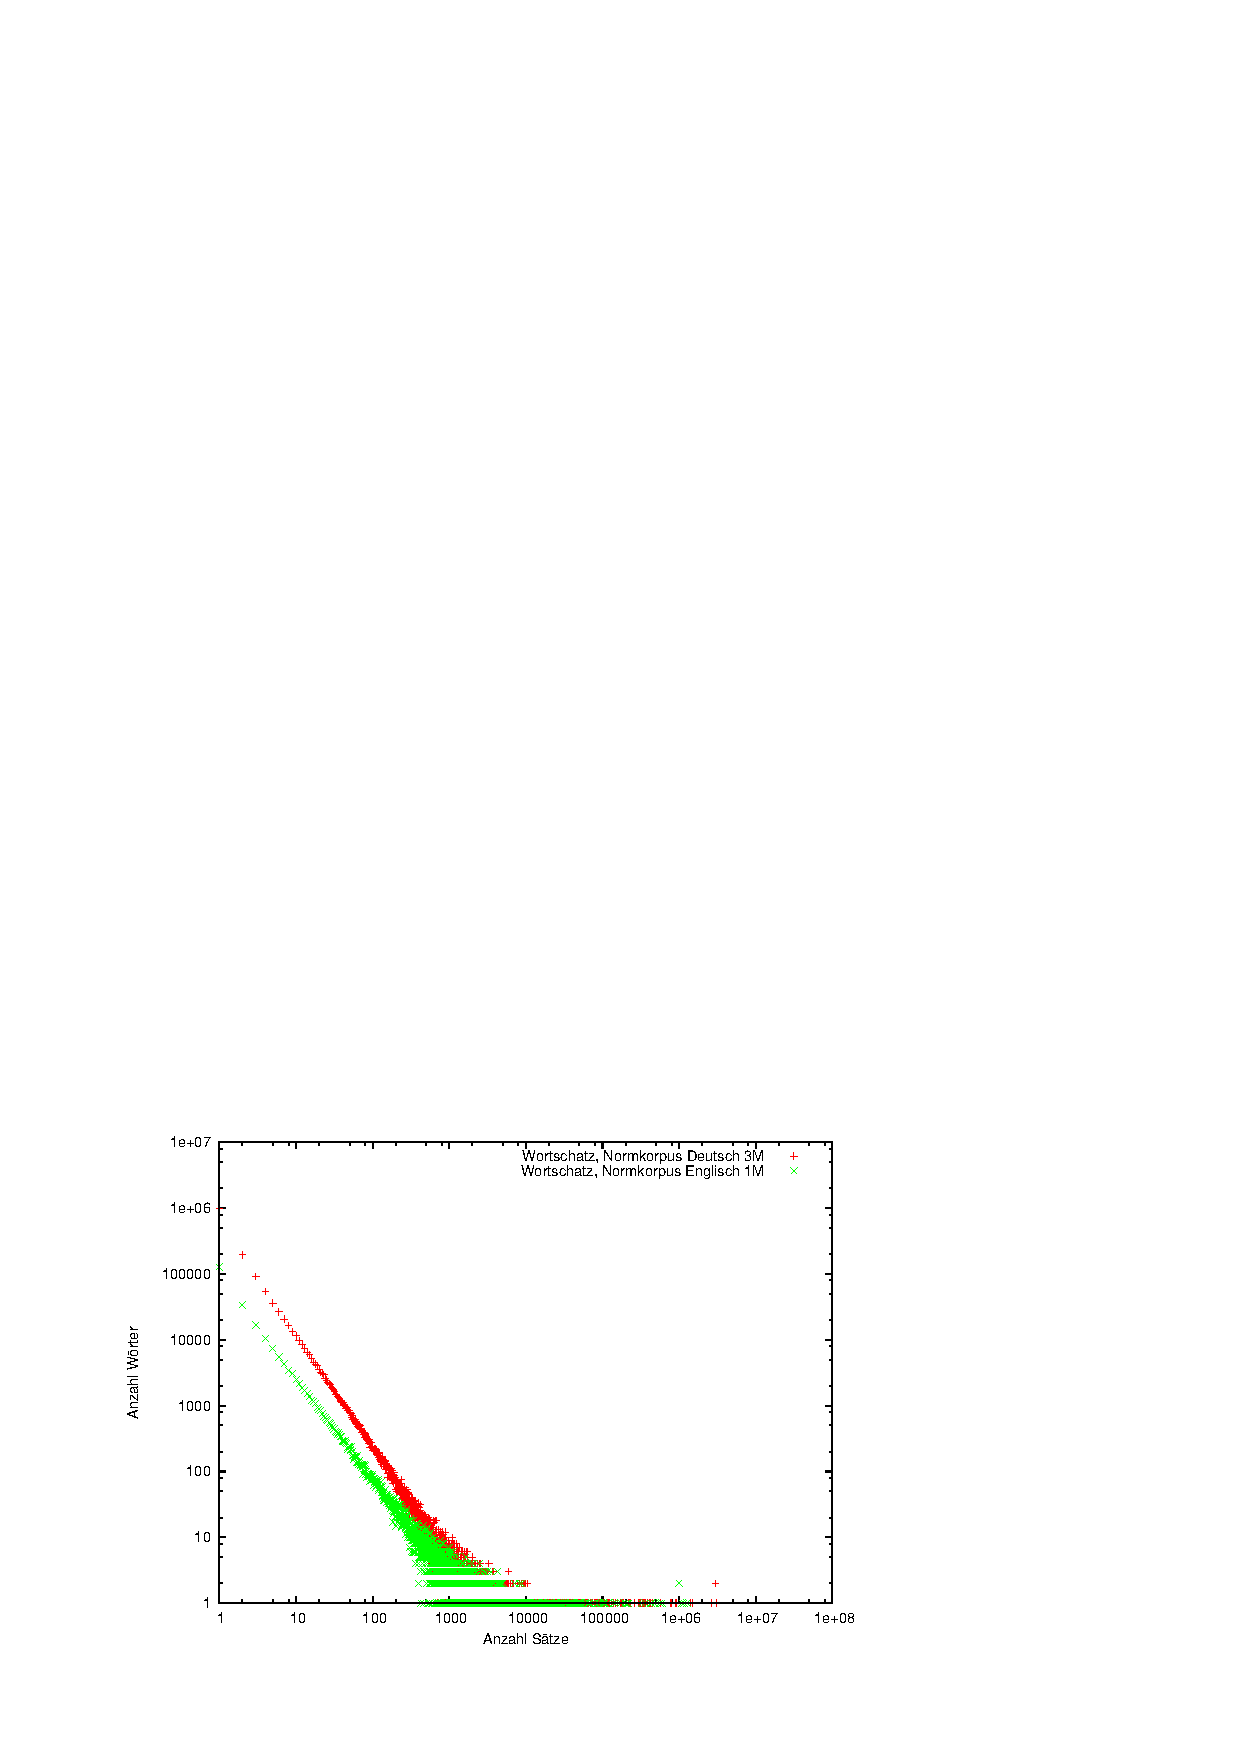
\includegraphics[width=\textwidth]{img/pdf/powerlaw_wortschatz.pdf}
%\caption{}
\label{fig:powerlaw_wortschatz}
\end{figure}

\begin{figure}[htb]
\includegraphics[width=1\textwidth]{img/pdf/zipf_wortschatz_reduced.pdf}
\caption[]{Frequenzverteilung in zwei ausgewählten Korpora}
\label{fig:zipf_wortschatz}
\end{figure}

\begin{figure}[htb]
\includegraphics[width=1\textwidth]{img/pdf/zipf_wortschatz_with_expected_values_reduced.pdf}
\caption[]{Vergleich mit einer idealen Verteilung nach dem Zipfschen Gesetz}% $\frac{f_{\max}}{Rang}$
\label{fig:zipf_wortschatz_with_expected_values}
\end{figure}

\begin{figure}[htb]
\includegraphics[width=1\textwidth]{img/pdf/zipf_wortschatz_frequency_class_reduced.pdf}
\caption[]{Aufteilung der Wortformen auf die verschiedenen Frequenzklassen}
\label{fig:zipf_wortschatz_frequency}
\end{figure}
\paragraph{} 
Die Daten des Wortschatzprojektes sind sowohl über ein Webportal\footnote{\url{http://corpora.informatik.uni-leipzig.de/}},
als auch per Download\footnote{\url{http://corpora.informatik.uni-leipzig.de/download.html}}
und als Webservice\footnote{\url{http://wortschatz.uni-leipzig.de/Webservices/}} verfügbar.

% dipl arbeit von christian biemann
% Seit 1994 wurde an der Universität Leipzig unter der Leitung von Uwe
% Quasthoff eine Infrastruktur erstellt, um elektronische Korpora zu
% analysieren und mit ihnen arbeiten zu können.
% Das inzwischen angesammelte Datenmaterial macht das :RUWVFKDW]-
% Korpus zu einem der größten Korpora in Deutsch, Englisch und
% Italienisch (je über 9 Mio. Sätze), desweiteren existieren noch kleinere
% Korpora in Französisch, Niederländisch und Sorbisch, sowie Korpora
% eingeschränkter Sachgebiete.
% Ziel bei der Erstellung war es, eine umfassende Datenbasis zu schaffen,
% um weitere Untersuchungen zu erleichtern. Die verarbeiteten Texte
% bestehen hauptsächlich aus einer Auswahl verschiedener Tageszeitungen,
% sowie Nachschlagewerken und von Verlagen für das Projekt freigegebenen
% Texten. Aus urheberrechtlichen Gründen dürfen die Texte nur satzweise
% gespeichert werden, weswegen der Satz die größte Einheit im Wortschatz
% darstellt.
% Auf die Rohdaten gestützt existieren verschiedene Datenbanken, die zur
% Strukturierung und als Vorarbeit für linguistische Algorithmen erstellt
% wurden. Als Vertreter seien hier die Kollokationsdatenbank, in der
%                                     -7-
% -
% Wortpaare,     die   signifikant  häufig    miteinander    in   Sätzen   oder
% nebeneinander auftreten, und die Datenbanktabelle 6DHW]H, die für alle
% indizierten Wörter Beispielsätze liefert, genannt.
% Im Gegensatz zum traditionellen Lexikon stellt die Wortschatz-Datenbank
% ein Vollformenlexikon dar, was sich aus der Konstruktion durch
% automatischen Aufbau ergibt. Hier gelten verschiedene Zeichenketten als
% verschiedene Wörter.
% Zum Datenbestand des deutschen Hauptkorpus gehören über 6 Millionen
% Wortformen,       über    36    Millionen    Sätze,   über    2,5   Millionen
% Grammatikangaben        sowie    Angaben     zur   Pragmatik,   Morphologie,
% Sachgebieten und weiteren Worteigenschaften.
% In einem Eintrag stehen die absolute Häufigkeit im Gesamtkorpus,
% Synonyme, Antonyme, Grammatikangaben, Sachgebiete, Beispielsätze und
% weiteres (siehe [Quasthoff 1998], [Quasthoff 2002a]).
% Der Wortschatz stellt einen Korpus im linguistischen Sinne dar: Bei der
% Auswahl der Texte wurde auf Vielfalt von Quellen und Sachgebieten
% geachtet, das Hauptkorpus wächst nicht weiter, liegt in maschinenlesbarer
% Form vor und ist mit eingeschränkten Suchmöglichkeiten im Internet seit
% März 1998 frei verfügbar.
\FloatBarrier

%\section{Ontology Learning}

%\section{Disambiguierung}
%\paragraph{Ähnlichkeitsmaß}\todo{...}
%Es handelt sich bei dieser Hierarchie um einen Baum

% %\chapter{State of the Art}
% \iffalse
% \section{Parser}
% Ein Parser für natürliche Sprachen ist ein Programm, welches die grammatikalische Struktur von Sätzen bestimmt und damit einen Syntaxbaum erstellt.
% In dieser Arbeit behandeln wir probabilistische Parser. Diese lernen die Struktur einer Sprache anhand von handannotierten Beispielen (einer Treebank) und
% erstellen dann bei Eingabe eines Satzes die Satzstruktur mit der höchsten Wahrscheinlichkeit. Auch wenn diese Art Parser noch ab und zu Fehler macht, funktionieren sie in der Praxis in den meisten Fällen sehr gut
% 
% \subsection{PCFG}
% A stochastic context-free grammar (SCFG; also probabilistic context-free grammar, PCFG) is a context-free grammar in which each production is augmented with a probability.
% The probability of a derivation (parse) is then the product of the probabilities of the productions used in that derivation;
% thus some derivations are more consistent with the stochastic grammar than others. SCFGs extend context-free grammars in the same way that hidden Markov models extend regular grammars.
% SCFGs have application in areas as diverse as Natural language processing to the study of RNA molecules. SCFGs are a specialized form of weighted context-free grammars.
% 
% Ein grundlegendes Problem der Lerntheorie ist, dass man theoretisch eine Sprache nicht nur aufgrund einer Menge positiver Beispiele (\zb{} einer Treebank) lernen kann.
% Wie Gold 1967 bewies\cite{gold67limit}, benötigen kontextfreie Grammatiken (und sogar schon Reguläre) zum Lernen sowohl positive als auch negative Beispiele.
% 
% Probabilistische kontextfreie Grammatiken können jedoch auch ausschließlich anhand von positiven Beispielen gelernt werden und erzielen in der Praxis damit sehr gute Ergebnisse.
% 
% Eine PCFG (probabilistische kontextfreie Grammatik) ist eine kontextfreie Grammatik, bei der jede Produktionsregel mit einer Wahrscheinlichkeit ausgezeichnet ist.
% Die Wahrscheinlichkeit einer Ableitung ist dann das Produkt der Wahrscheinlichkeiten der Produktionsregeln, die in der Ableitung vorkommen.
% Parst man nun einen Satz, der mehrere mögliche Ableitungen hat, dann kann man anhand der Wahrscheinlichkeiten dieser Ableitungen bestimmen, welcher dieser Syntaxbäume plausibler ist.
% Diese Plausibilitätseinschätzung ist allerdings nicht sehr gut, da sie nur auf der grammatischen Struktur des Satzes basiert und nicht darauf, welche Bedeutung des Satzes sinnvoller wäre.
% 
% 
% Laut\cite{accurate_unlexicalized_parsing} erreichten \todo{unlexicalized übersetzen} PCFG Parser im Test eine Genauigkeit von 86.36\% (LP/LR F1).
% 
% %\todo{übersetzt von \url{http://www.ps.uni-sb.de/~duchier/esslli-2000/node60.html#sec.dependency.formal}}
% \subsection{Phrasenstrukturgrammatik}
% Eine Phrasenstrukturgrammatik unterteilt einen Satz in eine hierarchische Gliederung aus sogenannten Phrasen oder Konstituenten.
% Sie ist sehr gut durch einen kontextfreie Grammatik repräsentierbar und \todo{was hierfür relevant ist}
% \todo{Bild}
% \subsection{Dependenzgrammatik}
% Eine Dependenzgrammatik (englisch Dependency Grammar) ist eine Grammatik, bei die Satzstruktur anhand von Abhängigkeiten von Wörtern untereinander dargestellt wird.
% Jedes Wort erzeugt eine bestimmte Zahl von Leerstellen im Text, es hat also eine bestimmte Valenz (Stelligkeit). Deshalb spricht man auch von einer Valenzgrammatik.
% Das zentrale Element eines Satzes in einer Dependenzgrammatik ist der sogenannte "`ultimative Head"', meist ein Verb.
% 
% Das Verb "`sehen"' etwa erwartet einen Sehenden und etwas Gesehenes.
% \begin{itemize}
%  \item "`Susi sieht die Sonne"' 
% \end{itemize}
% Andere Satzelemente kann man jedoch frei hinzufügen.
% \begin{itemize}
%  \item "`Susi sieht die Sonne, die heute sehr hell scheint."' 
% \end{itemize}
% \todo{Bild}
% 
% \paragraph{Vergleich}
% Hauptanliegen dieser Arbeit ist ja das Erlernen der charakteristischen Eigenschaften eines Satzes, um diesen gegen Andersartige abzugrenzen und Gemeinsamkeiten zu ähnlich Strukturierten zu finden.
% Da für jeden Grammatiktyp eine andere Ontologie erzeugt oder gefunden werden sowie ein Parser trainiert werden muss, ist es in dieser Arbeit aus Zeitgründen nicht möglich, beide zu integrieren und 
% hinsichtlich der Lernraten bei einigen häufigen Sprachfeatures zu analysieren. Aufgrund der modularen Struktur des Programmes ist es allerdings jederzeit nachrüstbar.
% Aus diesem Grund musste im Vorhinein eine Entscheidung gefällt werden, die zugunsten der Phrasenstrukturgrammatik ausfiel.
% Normalerweise werden Dependenzrepräsentationen für Sprachen mit großer Freiheit hinsichtlich der Wortreihenfolge (wie \zb{} Deutsch) empfohlen,
% Phrasenstrukturerepräsentationen werden hingegen für Sprachen mit festeren Satzstrukturen (wie \zb{} Englisch) vorgeschlagen.
% Trotzdem ist für beide Sprachen beides möglich. 
% \todo{Ist hier noch ein Beleg erforderlich? Wenn ja, dann Suchen und Einfügen, entnommen aus -> hier steht das drin http://www.ilc.cnr.it/EAGLES96/segsasg1/node44.html}
% 
% \begin{itemize}
%  \item 
%  \item Für das deutsche NEGRA Corpus existiert bereits eine Phrasenstrukturontologie 
%  \item Auch für das englische SUSANNE Corpus existiert bereits eine solche Ontologie
% \end{itemize}
% 
% 
% \cite{dependency_grammar_and_dependency_parsing} Dependency Grammar and Dependency Parsing
% 
% \iffalse
% Eine Dependancy Grammar ist ein 7-Tupel $<$Words, Cats, Args, Comps, Mods, Lexicon, Rules$>$.\\
% 
% \begin{tabular}{lp{12cm}}
% Words		&eine endliche Menge vollständig gebeugter Wörter\\
% Cats		&eine endliche Menge von Kategorien, \zb{} n (noun), det (determiner) oder vfin (finite verb)\\
% Args		&eine endliche Menge von "`agreement tuples"', \zb{} $<$masc sing 3 nom$>$\\
% Comps		&eine endliche Menge von "`complement roles"', \zb{} subject oder zu\_infinitive\\
% Mods		&eine endliche Menge von "`modifier roles roles"', \zb{} adj (adjective), welche disjunkt zu Comps ist. Wir schreiben $\textnormal{Roles} = \textnormal{Comps} \dotcup \textnormal{Mods}$.\\
% Lexicon		&eine endliche Menge von Lexikoneinträgen (siehe unten)\\
% Rules		&eine endliche Menge binärer Prädikate, indiziert mit den Rollenlabels $\varrho$, welche lokale grammatikalische Prinzipien ausdrücken. Für jedes $\varrho \in \textnormal{Roles}$ 
% gibt es ein $\Gamma_\rho \in \textnormal{Roles}$, sodass $\Gamma_\rho(w_1,w_2)$ anzeigt, ob eine Kante vom Vaterknoten $w_1$ zum Kindknoten $w_2$, die mit $\rho$ ausgezeichnet ist, existieren darf.\\
% \end{tabular}
% ~\\
% Ein lexikalischer Eintrag ist eine Wert-Attribut-Matrix mit der Signatur:
% 
% $
% \left[
% \begin{tabular}{cc}
% string	&Words\\
% cat	&Cats\\
% arg	&Agrs\\
% comps	&$2^\textnormal{Comps}$\\
% \end{tabular}
% \right]
% $\\
% Wenn $e$ ein Lexikoneintrag ist, dann ist string$(e)$ die vollständige Form des zugehörigen Wortes, cat$(e)$ dessen Kategorie, agr$(e)$ das agreement tuple und comps$(e)$ die Valenz ausgedrückt als 
% eine Menge von complement roles.
% 
% \subsubsection{Dependency Tree}
% Sei V eine Menge von Knoten, die wir mit den natürlichen Zahlen $\setN$ identifizieren.
% \fi
% 
% \iffalse
% \section{Disambiguierung}%\footnote{Im Englischen \emph{Word Sense Disambiguation}}
% Disambiguierung, im Englischen \emph{Word Sense Disambiguation}, beschäftigt sich damit, die Bedeutung eines Wortes in einem bestimmten Kontext herauszufinden.
% \begin{bsp}
% \emph{Hans setzte sich auf die Bank, denn die Sonne schien.}\\
% Welche Bedeutung hat das Wort \emph{Bank} in diesem Satz, ist hier das Möbelstück oder das Geldinstitut gemeint?
% \end{bsp}
% \subsection{Tiefer Ansatz}\todo{besser Übersetzen: deep approach}
% Dieser Ansatz setzt eine große Menge an Weltwissen vorraus. Hier könnte dies enthalten:
% "`Wenn die Sonne scheint, halten sich Menschen öfter in Parks auf. Parks enthalten oft Bänke (das Möbelstück). Auf eine Bank (das Möbelstück) kann sich ein Mensch setzen. Auf eine Bank (das Geldinstitut) kann sich ein
% Mensch nicht setzen"'.
% Das Problem bestand hier lange Zeit darin, dass außerhalb streng eingegrenzter Fachgebiete keine maschinenverarbeitbare Sammlung von Weltwissen verfügbar war.
% Es gab zwar Versuche, geschriebene Lexika maschinenlesbar aufzubereiten\cite{j:ewords}, dies brachte jedoch nur begrenzten Erfolg.
% Ein Quantensprung war dann jedoch das DBpedia-Projekt, das die riesige, sich ständig aktualisierende und erweiternde Wissensquelle Wikipedia automatisch zur Extraktion maschinenverarbeitbarer Daten nutzt.
% 
% These approaches are not very successful in practice, mainly because such a body of knowledge does not exist in a computer-readable format, outside of very limited domains. However, if such knowledge did exist, then deep approaches would be much more accurate than the shallow approaches.
% \fi
% \iffalse
% Deep approaches presume access to a comprehensive body of; world knowledge. Knowledge, such as "you can go fishing for a type of fish, but not for low frequency sounds"
%  and "songs have low frequency sounds as parts, but not types of fish", is then used to determine in which sense the word is used. These approaches are not very successful in practice, 
% mainly because such a body of knowledge does not exist in a computer-readable format, outside of very limited domains. However, if such knowledge did exist, then deep approaches would be 
% much more accurate than the shallow approaches. Also, there is a long tradition in computational linguistics, of trying such approaches in terms of coded knowledge and in some cases, it is
%  hard to say clearly whether the knowledge involved is linguistic or world knowledge. The first attempt was that by Margaret Masterman and her colleagues, at the Cambridge Language Research Unit in England,
% in the 1950s. This attempt used as data a punched-card version of Roget's Thesaurus and its numbered "heads", as an indicator of topics and looked for repetitions in text, using a set intersection algorithm.
%  It was not very successful, as is described in some detail in (Wilks, Y. et al., 1996), but had strong relationships to later work, especially Yarowsky's machine
%  learning optimisation of a thesaurus method in the 1990s.
% \fi\iffalse
% \subsection{Flache Ansätze}\todo{besser Übersetzen: shallow approach}
% \todo{material:}
% Preliminary Results in Tag Disambiguation using DBpedia
% 
% \cite{conf/naacl/Mihalcea07}
% \fi
% %\section{Ontology Learning}
% 
% %\section{Textklassifikation}
% \iffalse
% Rocchios Algorithmus
% 
% Rocchios Algorithmus basiert auf dem Relevanz-Feedback-Algorithmus.
% Er war einer der ersten RF-Algorithmen und wurde von J.J. Rocchio in \cite{rocchio_algorithm} vorgestellt.
% Relevanz-Feedback-Algorithmen sind eine effektive Möglichkeit, Benutzeranfragen zu erweitern oder zu verändern und daher \zb{} für Suchmaschinen sehr gut geegnet.
% Dabei wird die Anfrage schrittweise verfeinert, in dem aus allen als relevant oder irrelevant bekannten Dokumenten Merkmalsvektoren gebildet werden und aus diesen dann mit der folgenden Formel die nächste Anfrage
% berechnet wird:
% \[Q_j = \alpha Q_{j-1} + \frac{\beta}{N_R} \sum_{i=1}^{N_R} R_i + \frac{\gamma}{N_S} \sum_{i=1}^{N_S} S_i\]
% $Q_j$ ist dabei die Anfrage der Stufe $j$, $\alpha$, $\beta$ und $\gamma$ konstante Gewichtungen. $N_R$ ist die Anzahl relevanter, $N_S$ die Anzahl irrelevanter Dokumente. $(R_i)$ und $(S_i)$ sind die bereits
% als relevant bzw. irrelevant bestimmten Dokumente. $Q$, $R$ und $S$ sind dabei Vektoren von Termen aus einem Vektorraummodell. Aus dem resultierenden Anfragevektor werden sämtliche negativen Koeffizienten auf null gesetzt.
% Mit sämtlichen noch nicht eingestuften Dokumenten wird das Skalaprodukt zwischen dem Dokumentenvektor und dem Anfragevektor gebildet und nach dem Ergebnis ein Ranking gebildet, je höher das Skalarprodukt ist,
% desto höher die Relevanz des Ergebnisses. In einer Studie\cite{relevance_feedback_using_support_vector_machines} wird allerdings gezeigt, dass Rocchios Algorithmus schlecht abschneidet,
% wenn der Anteil relevanter Dokumente gering ist (wie es mittlerweile bei Spam der Fall ist,
% 
% \cite{a_hybrid_relevance-feedback_approach_to_text}
%                                             A recent study [3] revealed that
% Rocchio’s algorithm has a poor performance when the proportion of relevant
% documents in the whole corpus is quite low.
% \fi
% 
% \iffalse
% ****************BRIEF DESCRIPTION*********************
% 
% Rocchio’s Alogrithem
% 
% The Ricchio's Algorithm is based on the Relevancy Feedback Algorithms
% for Document Relevancy. Relevancy Feedback Models are an effective way
% of modifying and expanding user queries (such as search engines).
% 
% Ricchio's Algorithm is one of the earliest methods used for queries.
% This algorithm is basesd on the idea that if the relevance for a query
% is known, an optimal query vector will maximize the average
% query-document similarity for relevant documents, and will
% simultaneously minimize
% query-document similarity for non relevant documents. 
% 
% If we look at the basic formula for the Ricchio's Algorithm, the
% intuitive idea of Ricchio's Algorithm is to iteratively increase the
% weights of those terms contained in labeled relevant documents while
% penalizing the terms in the irrelevant documents.
% 
% Recent studies have shown that Ricchio's Algorithm has a poor
% performance when the proportion of relevant documents in the whole
% corpus is low.
% 
% http://www.cs.uml.edu/~kajal/courses/91.580-S03/papers/Hoashi.pdf
% http://www-student.cse.buffalo.edu/~arao/CSE741/slides.html
% http://ifsc.ualr.edu/xwxu/publications/ecir03_hybrid.pdf
% 
% 
% 
% 
% Naive Bayes
% 
% 
% 
% 
% Naive Byes algorithms are among the most successful known algorithms
% for learning to classify text documents. It predicts by reading a set
% of examples in attribute value-representation and than by using the
% Bayes Theorem to estimate the posterior probabilities of all
% qualifications. For each
% instance of the example language a classification with the highest
% posterier probability is chosen
% as the prediction. 
% 
% Example:
% 
% Suppose your data consist of fruits, described by their color and
% shape.  Bayesian classifiers operate by saying "If you see a fruit
% that is red and round, which type of fruit is it most likely to be,
% based on the observed data sample? In future, classify red and round
% fruit as that type of fruit."
% 
% A difficulty arises when you have more than a few variables and
% classes -- you would require an enormous number of observations
% (records) to estimate these probabilities.
% 
% Naive Bayes classification gets around this problem by not requiring
% that you have lots of observations for each possible combination of
% the variables.  Rather, the variables are assumed to be independent of
%  one another and, therefore the probability that a fruit that is red,
% round, firm, 3" in diameter, etc. will be an apple can be calculated
% from the independent probabilities that a fruit is red, that it is
% round, that it is firm, that is 3" in diameter, etc.
% 
% In other words, Naïve Bayes classifiers assume that the effect of an
% variable value on a given class is independent of the values of other
% variable. This assumption is called class conditional independence. It
% is made to simplify the computation and in this sense considered to be
% “Naïve”.
% 
% This assumption is a fairly strong assumption and is often not
% applicable.  However, bias in estimating probabilities often may not
% make a difference in practice -- it is the order of the probabilities,
% not their exact values, that determine the classifications.
% 
% Studies comparing classification algorithms have found the Naïve
% Bayesian classifier to be comparable in performance with
% classification trees and with neural network classifiers.  They have
% also exhibited high accuracy and speed when applied to large
% databases.
% 
% The problem with multinomial Naive Bayes is that when one class has
% more training examples than another, Naive Bayes selects poor weights
% for the decision boundary. This is due to an under-studied bias effect
% that shrinks weights for classes with few training examples. ANother
% systematic problem with Naive Bayes is that features are assumed to be
% independent. As a result, even when the words are dependent, each word
% contributes evidence individually. Thus the magnitude for the weights
% for classes with strong word dependencies is larger than for classes
% with weak word dependencies.
% 
% 
% http://www.wikipedia.org/wiki/Naive_Bayesian_classification
% http://www.dmg.org/pmmlspecs_v2/NaiveBayes.html
% http://www.cs.iastate.edu/~patterbj/cs/cs572/algs/naive.html
% http://www.resample.com/xlminer/help/NaiveBC/classiNB_intro.htm
% PORBLEMS WITH NAIVE BAYES
% http://www.ai.mit.edu/people/jrennie/papers/icml03-nb.pdf 
% 
% 
% 
% 
% K-Nearest Neighbor
% 
% 
% 
% 
% The goal of this clustering method is to simply separate the data
% based on the assumed similarities between various classes. Thus, the
% classes can be differentiated from one another by searching for
% similarities between the data provided.
% 
% The K-Nearest Neighbor is suitable for data streams. KNN does not
% build a classifier in advance. When a new sample arrives, KNN finds
% the K neighbors nearest to the new samples from the training space
% based on some suitable similarity or distance metric.
% 
% KNN is a good choice when simplicity and accuracy are the predominant
% issues. KNN can be superior when a  resident, trained and tested
% classifiers has a short useful lifespan, such as in the case with the
% data streams where new data is added rapidly and the training set is
% ever changing. KNN does not rely on prior probabilities, and it is
% computationally efficient. The main computation is the sorting of the
% training documents in order to find out the K nearest neighbors for
% the test document.
% 
% K-Nearest Neighbor is useful when their are less than 20 attributes
% per instance, there is lots of training data, training is very fast,
% learning complex target functions and don't want to loose information.
% The disadvantages of using such a function is that it is slow in
% sorting out queries and irrelevant attributes can fool the neighbor.
% 
% http://cs.hbg.psu.edu/~ding/publications/PAKDD02_KNN.pdf
% http://wwwcsif.cs.ucdavis.edu/~liaoy/research/text_ss02_html/node4.html
% http://www.cs.tufts.edu/~emower/KNN.html
% http://www4.cs.umanitoba.ca/~jacky/Teaching/Courses/74.436/current/Lectures/L07_Instance_Based_Learning.pdf
% 
% 
% 
% Decision Tree
% 
% 
% 
% The Decision Tree exploration engine, new to PolyAnalyst 4.1, helps
% solve the task of classifying cases into multiple categories. Decision
% Tree is PolyAnalyst's fastest algorithm when dealing with large
% amounts of  attributes. Decision Tree report provides an easily
% interpreted decision tree diagram and a predicted versus real table.
% 
% Problems to Solve: 
% 
% Classification of cases into multiple categories 
% 
% Target Attributes: 
% 
% Categorical or Boolean (Yes/No) attribute 
% 
% Output Format: 
% 
% Classification statistics 
% 
% Predicted versus Real table (confusion matrix) 
% 
% Decision Tree diagram 
% 
% Optimal Number of Records: 
% 
% Minimum of 100 records 
% 
% Maximum of 5,000,000 records 
% 
% Preprocessing Suggested: 
% 
% Summary Statistics - to deselect attributes that contain to many
% values to provide any useful insight to the exploration engine.
% 
% Underlying Algorithms: 
% 
% Information Gain splitting criteria 
% 
% Shannon information theory and statistical significance tests. 
% 
% The Data Used: 
% 
% Decision Tree works on data of any type. The DT algorithm is
% well-poised for analyzing very large databases  because it does not
% require loading all the data in machine main memory simultaneously.
% PolyAnalyst takes a  full advantage of this feature by implementing
% incremental DT learning with the help of the OLE DB for Data Mining
% mechanism.
% 
% The DT algorithm calculation time scales very well (grows only
% linearly) with increasing number of data columns. At the same time, it
% grows more than linearly with the growing number of data records - as
% N*log(N), where N is the number of records. Yet, for data of about
% 100,000 records, the DT algorithm is often the fastest exploration
% algorithm of PolyAnalyst.
% 
% Problems to Solve: 
% 
% Decision Tree algorithm helps solving the task of classifying cases
% into multiple categories. In many cases, this is the fastest, as well
% as easily interpreted machine learning algorithm of PolyAnalyst. The
% DT algorithm provides intuitive rules for solving a great variety of
% classification tasks ranging from predicting buyers/non-buyers in
% database marketing, to automatically diagnosing patient in medicine,
% and to determining customer attrition causes
% in banking and insurance. 
% 
% Target Attribute: 
% 
% The target attribute of a Decision Tree exploration must be of a
% Boolean (yes/no) or categorical data type.
% 
% When to Use This Algorithm: 
% 
% The Decision Tree exploration engine is used for task such as
% classifying records or predicting outcomes. You should use decision
% trees when you goal is to assign your records to a few broad
% categories. Decision Trees provide easily understood rules that can
% help you identify the best fields for further exploration.
% 
% The Output: 
% 
% The Decision Tree report starts of by giving measures resulting from
% the decision tree. These measures are the Number of non-terminal
% nodes, Number of leaves, and depth of the constructed tree. Next, the
% report provides classification statistics on the decision tree.
% 
% Problems:
% 
% The drawback of this algorithm is that large number of gini indices
% have to be computed at each node of the decision tree. In order to
% decide which attribute is to be split at each node, the gini indices
% have to be computed for all the attributes and for each successive
% pair of values for all patterns which have not been classified
% 
% OVERVIEW WITH AN EXAMPLE
% 
% http://www.bandmservices.com/DecisionTrees.htm
% 
% 
% 
% Support Vector Machine
% 
% 
% 
% A support vector machine is a supervised learning algorithm developed
% over the past decade by Vapnik and others (Vapnik, Statistical
% Learning Theory, 1998). The algorithm addresses the general problem of
% learning to discriminate between positive and negative members of a
% given class of n-dimensional vectors. For example, if you have a
% series of mRNA expression level measurements for each of a large
% number of genes, the SVM can learn to answer questions such as, ``Does
% the given gene belong to functional class X?'' where X is some
% category such as ``ribosomal genes'' or ``sugar and carbohydrate
% transporters.'' If you have a collection of digitized images of
% handwritten digits, the SVM can say whether a
% given image is, say, the number 9.
% 
% The SVM algorithm operates by mapping the given training set into a
% possibly high-dimensional feature space and attempting to locate in
% that space a plane that separates the positive from the negative
% examples. Having found such a plane, the SVM can then predict the
% classification of an unlabeled example by mapping it into the feature
% space and asking on which side of the separating plane the example
% lies. Much of the SVM's power comes from its criterion for selecting a
% separating plane when many candidates planes exist: the SVM chooses
% the plane that maintains a maximum margin from any point in the
% training set. Statistical learning theory suggests that, for some
% classes of well-behaved data, the choice of the maximum margin
% hyperplane will lead to maximal generalization when predicting the
% classification of previously unseen examples (Vapnik, Statistical
% Learning Theory, 1998). The SVM algorithm can also be extended to cope
% with noise in the training set and with multiple classes (Cristianini
% and Shawe-Taylor, An Introduction to Support Vector Machines, 2000).
% 
% Say that we have a training data set containing n examples, each of
% which is a vector of m numbers. These vectors may be thought of as
% points in an m-dimensional space. In theory, a simple way to build a
% binary classifier is to construct a hyperplane (i.e., a plane in a
% space with more than three dimensions) separating class members
% (positive examples) from non-members (negative examples) in this
% space. Unfortunately, most real-world problems involve non-separable
% data for which there does not exist a hyperplane that successfully
% separates the positive from the negative examples. One solution to the
% inseparability problem is to map the data into a higher-dimensional
% space and define a separating hyperplane there. This
% higher-dimensional space is called the feature space, as opposed to
% the input space occupied by the training examples. With an
% appropriately chosen feature space of sufficient dimensionality, any
% consistent training set can be made separable. However, translating
% the training set into a higher-dimensional space incurs both
% computational and learning-theoretic costs. Furthermore, artificially
% separating the data in this way exposes the learning system to the
% risk of finding trivial solutions that overfit the data.
% 
% SVMs elegantly sidestep both difficulties. They avoid overfitting by
% choosing the maximum margin separating hyperplane from among the many
% that can separate the positive from negative examples in the feature
% space. Also, the decision function for classifying points with respect
% to the hyperplane only involves dot products between points in the
% feature space. Because the algorithm that finds a separating
% hyperplane in the feature space can be stated entirely in terms of
% vectors in the input space and dot products in the feature space, a
% support vector machine can locate the hyperplane without ever
% representing the space explicitly, simply by defining a function,
% called a kernel function, that plays the role of the dot product in
% the feature space. This technique avoids the computational burden of
% explicitly representing the feature vectors.
% 
% http://www-ai.cs.uni-dortmund.de/SOFTWARE/SVM_LIGHT/svm_light_v3.02.eng.html
% http://www.afia.polytechnique.fr/CAFE/ECML01/SVM.html
% 
% 
% 
% Latent Semantic Analysis
% 
% 
% 
% Latent Semantic Analysis (LSA) analyzes word-word, word-passage, and
% passage-passage relationships. There's a good relationship between
% what LSA extracts and what people understand. LSA doesn't use
% first-hand knowledge of the world, but extracts from "episodes" of
% word content. LSA doesn't use word order or logic relationships. LSA
% uses unitary expressions of meaning instead of relationships between
% successive words. A word is a kind of average of meaning through all
% passages.
% 
% Dimensionality is reduced to approximate human cognition. LSA is a
% theory of knowledge representation. Dimensionality reduction solves
% the problem of "insufficient evidence" or "poverty of the stimulus".
% LSA uses a matrix decomposition algorithm to reduce the
% dimensionality. Ideally, the dimension of the reconstruction equals
% that of the passages. Results show that the meaning similarities are
% close to that of humans, LSA's rate of knowledge acquisition
% approximates that of humans, and LSA depends on the dimensionality.
% 
% LSA can be use to test theories of human cognition. LSA skips over the
% order of words to capture relationships in word choice. LSA uses a
% pre-processing step for word correlation over many passages and
% contexts. LSA uses a very large number of relationships. Theories of
% human cognition cannot be settled by theoretical and philosophical
% ideas.
% 
% LSA is an automatic mathematical algorithm for extracting
% relationships in word usage in passages. It doesn't use dictionaries,
% external knowledge, or grammar rules. First, represent words as a
% matrix, each row is a word, and each column is a text passage or
% context. Next, do a preliminary transformation of the matrix. Each
% word frequency in the Next, LSA applies singular value decomposition
% (SVD) to the matrix, which is factor analysis. The decomposition
% results in dimensionality reduction. Extract words from the passage
% into a word matrix, do a linear decomposition of the matrix, then
% reduce the dimensionality of the matrix. The LSA matrix adds words not
% in the passage, like human minor knowledge acquisition. LSA is
% intuitively sensible, with a three-fourths gain in total comprehension
% vocabulary inferred from knowledge about words not in the passage or
% paragraph. Human children have a rapid growth of vocabulary and
% knowledge. Humans draw conclusions from missing data. Reducing the
% dimensionality of representation is useful when the representation
% matches the data. The data should not be perfectly regenerated. The
% similarity of dimensionality reduction is the cosine between vectors.
% 
% Before the SVD is computed, LSA does a data preprocessing matrix data
% transformation. Save the log word frequency, and the entropy for each
% row and column of the word. Weight each word occurrence by an estimate
% of its importance in the passage. Knowing a word provides information
% about the passage it appeared in. Matrix transformations are used in
% information retrieval and human cognition models. A web site provides
% LSA based word or passage vectors, similarities between words and
% words, words and passages, and passages and passages. LSA is able to
% model human conceptual knowledge.
% LSA links information retrieval and human semantic memory. Latent
% Semantic Indexing (LSI), like LSA, was tested against pre-examined
% documents. Direct comparisons were muddied by preprocessing words. LSA
% does synonym tests, since most near neighbors are related by the
% cosine. LSA vectors were created from many passages. LSA captures
% synonymity by knowledge
% of captured vocabularies. TOEFL vocabulary simulates human performance
% between word choice. LSA errors were compared to student errors. The
% role of dimension reduction was analyzed. LSA simulates word sorting
% and word relationships. Subject-matter knowledge and sematic priming
% are in LSA. Predictive learning and text comprehension for humans.
% 
% http://www.uni-koblenz.de/~fruit/publications/Obst99c.html
% http://www.cs.toronto.edu/~psy/lsa.pdf 
% http://www.cs.nmsu.edu/~mmartin/LSA_Intro_AI_Seminar.ppt
% 
% RESOURCE
% 
% http://citeseer.nj.nec.com/563891.html
% 
% Voted Classification
% 
% http://216.239.39.104/search?q=cache:CcXO0h6c-Z4J:robotics.stanford.edu/users/ronnyk/vote.pdf+voted+classification+algorithm&hl=en&ie=UTF-8
% \fi